\documentclass[11pt,a4paper]{article}
\usepackage[T1]{fontenc}
\usepackage[utf8]{inputenc}
\usepackage{lmodern,microtype}
\usepackage[margin=22mm,top=23mm,bottom=23mm,headheight=14pt]{geometry}
\usepackage{amsmath,amssymb,mathtools}
\usepackage{booktabs,tabularx,array,longtable}
\usepackage[dvipsnames]{xcolor}
\usepackage{enumitem,fancyhdr,titlesec}
\usepackage[most]{tcolorbox}
\usepackage{listings}
\usetikzlibrary{arrows.meta}
\usepackage{hyperref,xurl}
\definecolor{ink}{HTML}{182D42}
\definecolor{accent}{HTML}{007D86}
\definecolor{muted}{HTML}{546475}
\definecolor{pale}{HTML}{EEF5F6}
\hypersetup{colorlinks=true,linkcolor=accent,citecolor=accent,urlcolor=accent,
 pdftitle={N=2 theories: mathematical background and implementation reference},
 pdfauthor={SuperconformalIndex project},bookmarksnumbered=true}
\titleformat{\section}{\Large\sffamily\bfseries\color{ink}}{\thesection}{0.7em}{}
\titleformat{\subsection}{\large\sffamily\bfseries\color{ink}}{\thesubsection}{0.6em}{}
\titleformat{\subsubsection}{\normalsize\sffamily\bfseries\color{accent}}{}{0em}{}
\titlespacing*{\section}{0pt}{0pt}{14pt}
\titlespacing*{\subsection}{0pt}{13pt}{8pt}
\titlespacing*{\subsubsection}{0pt}{10pt}{5pt}
\setlength{\parindent}{0pt}
\setlength{\parskip}{6pt}
\setlength{\emergencystretch}{2em}
\setlist{itemsep=3pt,topsep=4pt,leftmargin=1.5em}
\renewcommand{\arraystretch}{1.2}
\newcolumntype{Y}{>{\raggedright\arraybackslash}X}
\numberwithin{equation}{section}
\pagestyle{fancy}
\fancyhf{}
\fancyhead[L]{\small\sffamily\color{muted}SUPERCONFORMALINDEX / REFERENCE}
\fancyhead[R]{\small\sffamily\color{muted}10 September 2026}
\fancyfoot[L]{\footnotesize\color{muted}Mathematics \& implementation \enspace | \enspace consolidated edition}
\fancyfoot[R]{\small\thepage}
\renewcommand{\headrulewidth}{0.3pt}
\newcommand{\code}[1]{{\small\nolinkurl{#1}}}
\BeforeBeginEnvironment{tabularx}{\par\noindent}
\AfterEndEnvironment{tabularx}{\par}
\newcommand{\file}[1]{\par{\small\sffamily\color{muted}MODULE \quad\texttt{\detokenize{#1}}}\par}
\newcommand{\PE}{\operatorname{PE}}
\newcommand{\PL}{\operatorname{PL}}
\newcommand{\Tr}{\operatorname{Tr}}
\newcommand{\rank}{\operatorname{rank}}
\newcommand{\adj}{\mathrm{adj}}
\newcommand{\CB}{\mathrm C}
\newcommand{\HL}{\mathrm{HL}}
\newcommand{\QQ}{\mathbb Q}
\newcommand{\CC}{\mathbb C}
\newcommand{\ZZ}{\mathbb Z}
\newcommand{\src}[1]{{\small\color{muted}Source: #1.}\par}
\newtcolorbox{note}[1]{enhanced,breakable,colback=pale,colframe=accent,
 boxrule=0pt,borderline west={2pt}{0pt}{accent},arc=0pt,
 left=10pt,right=10pt,top=7pt,bottom=7pt,title={#1},
 coltitle=ink,fonttitle=\sffamily\bfseries,attach title to upper={\par\smallskip}}
\lstset{basicstyle=\ttfamily\footnotesize,columns=fullflexible,keepspaces=true,
 breaklines=true,breakatwhitespace=false,showstringspaces=false,
 backgroundcolor=\color{pale},frame=single,rulecolor=\color{pale},
 xleftmargin=5pt,xrightmargin=5pt,aboveskip=8pt,belowskip=8pt}

\begin{document}
\hypersetup{pageanchor=false}
\begin{titlepage}
\vspace*{13mm}
{\sffamily\color{accent}\large SUPERCONFORMALINDEX}\par
\vspace{10mm}
{\sffamily\bfseries\color{ink}\Huge $\mathcal N=2$ theories}\par
\vspace{5mm}
{\sffamily\color{ink}\LARGE Mathematical background\par and implementation reference}\par
\vspace{12mm}
{\Large One reference, organized by package}\par
\vspace{6mm}
Exact Lie-algebra data, anomaly checks, superconformal indices,\par
Coulomb-branch indices and spectra, theory properties,\par
database persistence, and the planned Higgs-branch extension.
\vspace{11mm}
\begin{note}{Index/cache update: reusable expansions and decompositions}
Exact FORM expansions are now stored by raw program text. Character products
reuse cached lower-order factors, and a process-pool builder prepares every
product through a chosen weighted Adams order. This edition explains the
cutoff proof, APIs, concurrency and measured performance, with current validation.
The database chapter retains the schema-version-6 reference.
\end{note}
\vfill
\begin{tabularx}{\textwidth}{@{}p{31mm}Y@{}}
Snapshot & Base reference: 8 September 2026. Database and validation update:
9 September 2026. Index/cache update: 10 September 2026; \code{04bbe21}.\\
Consolidates & \code{index/n2_theory_index_Mathematical_Background.pdf}\newline
and the previous \code{output/pdf/n2_implementation_reference_summary.pdf}.\\
Status & FORM expansion persistence, cached-factor planning and complete Adams
cache builder documented, with measured comparisons and the 209-test snapshot. Database structure retains its version-6 update; unrelated package
chapters retain the base reference snapshot.
Higgs/Hall--Littlewood material is explicitly marked as proposed, not implemented.\\
Editing scope & Documentation only. The companion index-background PDF is also
updated. Unrevised mathematical and package content is preserved.\\
\end{tabularx}
\end{titlepage}
\hypersetup{pageanchor=true}

\section{Project map and conventions}\label{sec:map}
\begin{tabularx}{\textwidth}{@{}p{25mm}Yp{21mm}@{}}
\toprule
Package & Responsibility & Read here\\\midrule
\code{anomalies} & Cartan types, representations, full/half hypers, beta functions,
local and conventional mod-two gauge anomalies. & \S\ref{sec:anomalies}\\
\code{index} & FORM expansion, LiE partial decompositions and SQLite singlet cache; Coulomb PE/PL and
full-index projection; future Higgs/flavor refinement. & \S\ref{sec:index}\\
\code{common} & Property orchestration, flavor blocks, central charges, exact-number
and FORM helpers, JSON and MySQL persistence. & \S\ref{sec:common}\\
\code{test} & Unit and backend regression tests, precision and serialization checks,
optional live database integration. & \S\ref{sec:test}\\\bottomrule
\end{tabularx}

\subsection*{How data moves}
\begin{center}
\fcolorbox{accent}{pale}{\parbox{0.89\textwidth}{\centering
Theory dictionary / JSON\quad$\longrightarrow$\quad validated gauge and hyper data\\[5pt]
$\longrightarrow$\quad anomaly and conformality checks\\[5pt]
$\longrightarrow$\quad properties, full index, Coulomb index and spectrum\\[5pt]
$\longrightarrow$\quad exact JSON and optional MySQL storage}}
\end{center}
Standalone index functions are also callable directly. The property and database
workflows impose the SCFT-candidate checks; a gauge-invariant counting calculation
alone is not a proof that an input defines an SCFT.

\subsection*{Notation used throughout}
\begin{tabularx}{\textwidth}{@{}p{30mm}Y@{}}
$G=\prod_{a=1}^{s}G_a$ & Compact, simply connected, semisimple gauge group; no abelian
gauge factor or global quotient is implemented.\\
$\mathcal R_h=\boxtimes_a R_{ha}$ & One product-group hyper representation;
$n_h$ is its number of copies. Omitted factors are singlets.\\
$\epsilon_h=1,\,\tfrac12$ & Weight of a full or half hyper, respectively. Beta
functions use $2\epsilon_h T$, not $\epsilon_h T$.\\
$E,R,r;j_1,j_2$ & Scaling dimension, $SU(2)_R$ weight, $U(1)_r$ charge, and Lorentz
Cartan weights in the chosen right-index convention.\\
$t,y,u$ & Project full-index fugacities; the common literature variable $v=u^2$.\\
$x$, $\tau$, $q$ & Coulomb grading, proposed HL grading, and an internal FORM
integer-power variable. This $q$ is not a conventional full-index fugacity.\\
\end{tabularx}

\begin{note}{What ``spectrum'' means here}
The Coulomb spectrum is the multiset of dimensions of independent chiral-ring
generators, with repetitions. Index coefficients count all graded ring elements,
including products. Neither is the spectrum of massive BPS particles or the full
operator spectrum of the SCFT.
\end{note}

\clearpage
\section{Package \texttt{anomalies}}\label{sec:anomalies}
\subsection{Root data and representation invariants}
\file{anomalies/lie_algebra.py}
\code{SimpleLieAlgebra} collects Sage root, weight and character objects together
with the rank, dimension, dual Coxeter number and adjoint Dynkin labels. The
cached constructor is \code{get_lie_algebra}. The accepted finite types are
$A_r$ ($r\geq1$), $B_r,C_r$ ($r\geq2$), $D_r$ ($r\geq4$),
$E_{6,7,8}$, $F_4$, and $G_2$. Use $A_1$ for $B_1/C_1$, $A_3$ for $D_3$,
and $A_1\times A_1$ for $D_2$.

For a dominant integral highest weight $\lambda$, Dynkin labels and dimensions are
\begin{align}
 \lambda&=\sum_i a_i\omega_i,&
 a_i&=\langle\lambda,\alpha_i^\vee\rangle\in\ZZ_{\geq0},\label{eq:dynkin}\\
 \dim V_\lambda&=\prod_{\alpha>0}
 \frac{(\lambda+\rho,\alpha)}{(\rho,\alpha)},&
 \rho&=\frac12\sum_{\alpha>0}\alpha.\label{eq:weyl-dim}
\end{align}
The algebra dimension is $\dim\mathfrak g=\rank\mathfrak g+|\Phi|$, and the
adjoint highest weight is the highest root. \code{representation_dimension}
uses the degree of the Sage Weyl character, implementing \eqref{eq:weyl-dim}.
\src{Sage root-system and Weyl-character documentation \cite{sage-roots,sage-chars}}

To compensate for the ambient root-length convention used by Sage, the code uses
\begin{equation}
 C_2(\lambda)=\frac{(\lambda,\lambda+2\rho)}{\ell_{\mathrm{long}}^2},
 \qquad T(R)=\frac{\dim R}{\dim\mathfrak g}C_2(R).
 \label{eq:casimir}
\end{equation}
If long roots have squared length two, the first denominator is two. Thus
$C_2(\adj)=T(\adj)=h^\vee$ and $T(\mathbf N)=1/2$ for $SU(N)$.
The routines are \code{quadratic_casimir} and \code{dynkin_index}.
The physics normalization is fixed by
$\Tr_R(T^aT^b)=T(R)\delta^{ab}$.

\subsubsection{Names, conjugation and reality}
\code{named_representation_labels} supports common names such as fundamental,
antifundamental, adjoint, singlet, classical spinors and selected two-index
representations. Explicit Dynkin labels are the general interface. Numbering is
Sage's finite-Cartan numbering; do not copy a label tuple from another reference
without checking its node convention.
\begin{equation}
 \lambda^*=-w_0\lambda,\qquad
 \nu(R)=\int_G\chi_R(g^2)\,d\mu(g)\in\{+1,0,-1\}.
 \label{eq:reality}
\end{equation}
Here $\nu=+1,0,-1$ means real, complex, pseudoreal.
\code{conjugate_dynkin_labels} uses the dual character;
\code{representation_reality} uses its Frobenius--Schur indicator.
For an irreducible external tensor product, $\nu(\boxtimes_aR_a)=\prod_a\nu(R_a)$.
\src{Sage Weyl characters \cite{sage-chars}; representation and index conventions
can be cross-checked with LieART 2.0 \cite{lieart}}

\clearpage
\subsection{Theory data, hypermultiplets and the beta function}
\file{anomalies/check_n2_anomalies.py}
The general input parser constructs \code{GaugeFactorData(factor_id, algebra)}
objects and simple/product hyper data. Counts are exact nonnegative integers.
Malformed types, labels or representations are rejected before calculation.
The theory dictionary supports either one simple factor or a list of named gauge
factors with a representation for each charged factor.

In $\mathcal N=1$ language, a full hyper in $\mathcal R$ contains chirals in
$\mathcal R\oplus\overline{\mathcal R}$. A half hyper contains one chiral and is
allowed only when the \emph{entire} gauge representation is pseudoreal.
Consequently $\mathbf2\boxtimes\mathbf2$ of $SU(2)^2$ is real and cannot be
a single half hyper, whereas $\mathbf2\boxtimes\mathbf2\boxtimes\mathbf2$ is
pseudoreal and can. This is validated rather than inferred from one factor alone.
\src{Bhardwaj--Tachikawa, \S2, Eqs.~(2.1)--(2.4) \cite{bt}}

For factor $a$, spectator dimensions multiply the effective number of charged
degrees of freedom. In the normalization of \eqref{eq:casimir},
\begin{equation}
 b_{0,a}=2h_a^\vee-
 \sum_h n_h\,(2\epsilon_h)\,T_a(R_{ha})
 \prod_{b\ne a}\dim R_{hb}.
 \label{eq:beta}
\end{equation}
The implementation uses the literal coefficient two for full hypers and one for
half hypers. $b_{0,a}=0$ for every simple factor is its one-loop conformality
condition; $b_{0,a}>0$ denotes asymptotic freedom in this convention.
\src{Bhardwaj--Tachikawa, Eqs.~(2.5)--(2.8) \cite{bt}}

\subsubsection{Checks that expose normalization mistakes}
For $SU(N)$ with $N_f$ full fundamental hypers,
\begin{equation}
 b_0=2N-N_f.
 \label{eq:sqcd-beta}
\end{equation}
For one full bifundamental $(\mathbf N,\mathbf M)$ of $SU(N)\times SU(M)$,
its contributions to the two beta-function subtractions are $M$ and $N$.
For a half hyper in an $SU(2)$ fundamental, the subtraction is $1/2$.
These follow directly from \eqref{eq:beta}, not from a new convention for $T$.

\begin{note}{Two different uses of ``index''}
The Dynkin index $T(R)$ is a quadratic trace invariant. It is unrelated to the
superconformal index $\mathcal I$. LieART's commonly tabulated quadratic index
$\ell(R)$ in the old project comparison is $2T(R)$; convert the convention
before comparing tables. Root/node numbering must be converted independently.
\end{note}

\subsubsection{Scope of the candidate flag}
The anomaly checker combines valid matter, gauge-anomaly cancellation and
vanishing beta functions into a \code{lagrangian_scft_candidate} result.
It does not reconstruct a Seiberg--Witten geometry, identify S-dual theories,
classify line operators, or handle non-Lagrangian matter sectors.

\clearpage
\subsection{Local and conventional global gauge anomalies}
For a left-handed Weyl fermion in $R$, the local cubic anomaly tensor is
\begin{equation}
 d_R^{abc}=\Tr_R\!\left(T^a\{T^b,T^c\}\right),\qquad
 d_{\overline R}^{abc}=-d_R^{abc}.
 \label{eq:cubic}
\end{equation}
Full hypers cancel between $R$ and $\overline R$; self-conjugate real or
pseudoreal representations have zero cubic tensor. The adjoint gauginos are in
a real representation. Thus local anomaly cancellation follows structurally for
the allowed matter schema; the checker need not tabulate every cubic invariant.
For semisimple product groups, mixed tensors with one generator from another
factor vanish by $\Tr T^a=0$.
\src{Bilal, discussion of chiral fermions, conjugate representations and anomaly
traces \cite{bilal}; matter restrictions in \cite{bt}}

\subsubsection{The mod-two test}
For factors with the conventional four-dimensional Witten anomaly, the number
of anomalous Weyl representations must be even. The code checks $A_1$, all
supported $C_r$, and $B_2\simeq C_2$. In its normalization the parity is
\begin{equation}
 \mathfrak a_a=
 \sum_{h\ \mathrm{half}} n_h\,[2T_a(R_{ha})]
 \prod_{b\ne a}\dim R_{hb}\pmod2.
 \label{eq:witten}
\end{equation}
Full hypers contribute an even number automatically. The integer entering this
test is $2T$, not the full-hyper beta contribution with an additional factor of
two. A nonzero parity makes the gauge theory inconsistent within this setup.
\src{Witten \cite{witten}; Wang--Wen--Witten, \S2.3 \cite{www};
symplectic-group discussion in \cite{bt,df}}

For $SU(2)$ isospin $j$, a useful independent formula is
\begin{equation}
 T_j=\frac13j(j+1)(2j+1),\qquad
 2T_j=\frac23j(j+1)(2j+1).
 \label{eq:su2-index}
\end{equation}
It is odd for $j=2k+1/2$, $k\in\ZZ_{\geq0}$: $j=1/2,5/2,9/2,\ldots$.
One fundamental half hyper is anomalous, two are safe. A single
$SU(2)^3$ trifundamental half hyper gives four doublets to each factor and is
safe under this conventional test, although it is not by itself conformal.

\begin{note}{Not an all-background anomaly classification}
The project assumes the ordinary spin-theory setting and simply connected
groups. It does not implement the newer non-spin $SU(2)$ anomaly associated with
isospin $4k+3/2$, global quotients, discrete theta angles or general bordism
anomalies. Flavor 't Hooft anomalies need not vanish and are not gauge-anomaly
rejection criteria. See \cite{www,df} for the distinction.
\end{note}

\clearpage
\subsection{Independent \texorpdfstring{$SU(N)$}{SU(N)} formula checks}
This section retains the useful representation-theory cross-checks from the
older reference. They are derived checks, not a second implementation backend.
For Dynkin labels $(a_1,\ldots,a_{N-1})$, define row lengths and box count by
\begin{equation}
 \ell_i=\sum_{k=i}^{N-1}a_k\quad(i<N),\qquad
 \ell_N=0,\qquad B=\sum_{i=1}^N\ell_i.
 \label{eq:rows}
\end{equation}
Specializing the Weyl dimension and highest-weight Casimir formulas gives
\begin{align}
 \dim R&=\prod_{1\leq i<j\leq N}
 \frac{\ell_i-\ell_j+j-i}{j-i},\label{eq:su-dim}\\
 C_2(R)&=\frac12\left[
 NB+\sum_{i=1}^N\ell_i(\ell_i+1-2i)-\frac{B^2}{N}\right],\label{eq:su-casimir}\\
 T(R)&=\frac{\dim R}{N^2-1}C_2(R).\label{eq:su-t}
\end{align}
\src{Direct specialization of \eqref{eq:weyl-dim} and \eqref{eq:casimir}; compare
Sage characters \cite{sage-chars} and representation tables in \cite{lieart}}

\begin{tabularx}{\textwidth}{@{}Yccc@{}}
\toprule
$SU(N)$ representation & Dimension & $C_2$ & $T$\\\midrule
Fundamental & $N$ & $(N^2-1)/(2N)$ & $1/2$\\
Adjoint & $N^2-1$ & $N$ & $N$\\
Two-index symmetric & $N(N+1)/2$ & $(N-1)(N+2)/N$ & $(N+2)/2$\\
Two-index antisymmetric & $N(N-1)/2$ & $(N+1)(N-2)/N$ & $(N-2)/2$\\
\bottomrule
\end{tabularx}
One symmetric plus one antisymmetric full hyper therefore gives
$2T_{\mathrm{sym}}+2T_{\mathrm{asym}}=2N$ and $b_0=0$.
For $N=2$ the antisymmetric is a singlet, with zero $T$.

\subsubsection{Function-to-equation map}
\begin{tabularx}{\textwidth}{@{}Yp{43mm}@{}}
\toprule Routine & Mathematical object\\\midrule
\code{get_lie_algebra}, \code{validate_dynkin_labels} & Root data and \eqref{eq:dynkin}\\
\code{representation_dimension} & \eqref{eq:weyl-dim}, checked by \eqref{eq:su-dim}\\
\code{quadratic_casimir}, \code{dynkin_index} & \eqref{eq:casimir}\\
\code{conjugate_dynkin_labels}, \code{representation_reality} & \eqref{eq:reality}\\
Gauge-factor beta calculation & \eqref{eq:beta}\\
Gauge-anomaly checks & \eqref{eq:cubic}, \eqref{eq:witten}\\\bottomrule
\end{tabularx}

\clearpage
\section{Package \texttt{index}}\label{sec:index}
\subsection{Full-index convention and single-letter functions}
\file{index/n2_theory_index.py}
In radial quantization the chosen right-handed supercharge restricts the trace to
\begin{align}
 \delta_R&=E-2j_2-2R+r=0,\label{eq:delta}\\
 \mathcal I(t,y,u)&=\Tr_{\delta_R=0}(-1)^F
 t^{2(E+j_2)}y^{2j_1}u^{-2(r+R)}.\label{eq:full-trace}
\end{align}
This is the literature convention with $v=u^2$. It is a signed protected trace,
not a positive count of every short multiplet: cancellations and recombination
mean the full operator spectrum cannot generally be recovered uniquely.
\src{Gadde--Pomoni--Rastelli, Eqs.~(5.4)--(5.5) \cite{gpr}}

Writing $D(t,y)=(1-t^3y)(1-t^3/y)$, the scalar coefficients of the vector and
half-hyper characters are
\begin{align}
 f_V(t,y,u)&=\frac{t^2u^2-t^4u^{-2}-t^3(y+y^{-1})+2t^6}{D(t,y)},
 \label{eq:vector-letter}\\
 f_H(t,y,u)&=\frac{t^2/u-t^4u}{D(t,y)}.\label{eq:hyper-letter}
\end{align}
The denominator counts the two allowed spacetime derivatives; fermionic letters
and equations of motion produce the numerator signs.
\src{Gadde--Pomoni--Rastelli, Eqs.~(5.21)--(5.22), with $v=u^2$ \cite{gpr}}

For gauge variables $g=(g_1,\ldots,g_s)$, the complete letter function is
\begin{equation}
 L=f_V\sum_a\chi_{\adj_a}(g_a)
 +f_H\left[\sum_{h\ \mathrm{full}}n_h
 (\chi_{\mathcal R_h}+\chi_{\overline{\mathcal R_h}})
 +\sum_{h\ \mathrm{half}}n_h\chi_{\mathcal R_h}\right].
 \label{eq:total-letter}
\end{equation}
Here $\chi_{\mathcal R_h}(g)=\prod_a\chi_{R_{ha}}(g_a)$.
The conjugate of a product representation conjugates every factor simultaneously:
$(R,S)\mapsto(\overline R,\overline S)$. A full bifundamental is not four
independent choices of conjugation. For a self-conjugate full hyper, the two
equal characters still give multiplicity two.

\begin{note}{Flavor-unrefined does not mean flavor-singlet}
All flavor fugacities are currently set to one. Flavor representations are
replaced by their dimensions, while gauge representations are kept until singlet
projection. Charged flavor operators are counted; the code does not project them
out. Spin and R-symmetry fugacities $y,u$ are still present.
\end{note}

\clearpage
\subsection{Plethystic expansion and FORM truncation}
For a letter function with no degree-zero term, define
\begin{equation}
 \PE[L]=\exp\!\left[\sum_{k\geq1}\frac1k
 L(t^k,y^k,u^k;g_1^k,\ldots,g_s^k)\right],\qquad
 \mathcal I=\int_G d\mu(g)\,\PE[L].
 \label{eq:full-pe}
\end{equation}
Adams substitution acts on every fugacity and character, but leaves numerical
multiplicities and the signed letter coefficients as coefficients. The Haar
measure is normalized so $\int_G1=1$.
\src{Plethystics \cite{plethystics}; gauge-index construction in \cite{gpr}}

\code{_character_basis} assigns formal character functions
$C_p(k)=\chi_{R_p}(g_a^k)$ to simple-factor irreps.
\code{_build_form_program} constructs the truncated exponent
\begin{equation}
 A_D=\left[\sum_{k=1}^{\lfloor D/2\rfloor}\frac{L(t^k,y^k,u^k;g^k)}k
 \right]_{t^{\leq D}}.
 \label{eq:trunc-exponent}
\end{equation}
Every letter begins at $t^2$, so $k>\lfloor D/2\rfloor$ and particle number
$m>\lfloor D/2\rfloor$ cannot contribute. Derivatives are expanded as
\begin{equation}
 D(t,y)^{-1}=\sum_{p,q\geq0}t^{3(p+q)}y^{p-q};
 \qquad p,q\leq\lfloor D/3\rfloor
 \label{eq:derivatives}
\end{equation}
is a sufficient rectangular bound before final degree truncation. FORM declares
$t$ with maximum power $D$, so excess combined powers are discarded throughout
the calculation. Negative powers of $u$ and $y$ are allowed.

\subsubsection{The auxiliary-variable recurrence}
The code starts with $zA_D$ and successively substitutes
\begin{equation}
 z\longmapsto1+\frac{zA_D}{m},\qquad m=2,\ldots,M,
 \quad M=\lfloor D/2\rfloor.
 \label{eq:exp-recursion}
\end{equation}
After step $m$, the expression is
$\sum_{j=1}^{m-1}A_D^j/j!+zA_D^m/m!$. Setting $z=1$ and adding the vacuum
term gives $\sum_{j=0}^{M}A_D^j/j!$ exactly through degree $D$.
This is the algebraic reason for the generated FORM substitutions, rather than
an approximation requiring a convergence assumption.
\src{Recurrence derived from the source; FORM syntax and truncation conventions
in the supplied FORM 5 manual \cite{form5}, with software background in \cite{form4}}

\code{run_form} is imported from \code{common/form_utils.py}.
\code{FormExpansionCache.parse_form_output} in \code{index/form_expansion_cache.py}
converts rational coefficients, fugacity exponents and character powers into
\code{IndexFormTerm} records. \code{get_expansion} reuses their SQLite serialization
when the complete raw FORM program is already cached. The numerical coefficients remain
exact rationals, including cancellations generated by the index.

\clearpage
\subsection{Gauge singlets, LiE and the reusable character cache}
\file{index/char_decomposition_cache.py}
The Adams operation is
\begin{equation}
 \psi^k\chi_R(g)=\chi_R(g^k),\qquad
 \prod_{k\geq1}(\psi^k\chi_R)^{n_k}
 =\sum_\lambda c_\lambda\chi_\lambda.
 \label{eq:adams}
\end{equation}
The right-hand side may be a \emph{virtual} character: $c_\lambda$ need not be
nonnegative. For $SU(2)$,
$\psi^2\chi_{\mathbf2}=\chi_{\mathbf3}-\chi_{\mathbf1}$, while
$\chi_{\mathbf2}^2=\chi_{\mathbf3}+\chi_{\mathbf1}$. Replacing the former with
the latter would change the PE and corrupt gauge projection.
\src{LiE manual, character operations \cite{lie}; Sage character operations
\cite{sage-chars}}

A full-decomposition request identifies the Cartan type, Dynkin labels and the
complete Adams-power tuple. Its weighted order is
\begin{equation}
 w=\sum_{k\geq1}k n_k.
 \label{eq:adams-order}
\end{equation}
This is metadata, not a unique key: $(2,0)$ and $(0,1)$ have the same order but
describe different virtual characters. Full decompositions remain available
through \code{get_decomposition}; singlet requests use the smaller calculation below.

Normalized Haar integration and the product-group rule are unchanged:
\begin{equation}
 \int_{G_a}\chi_\lambda(g_a)\,d\mu_a=\delta_{\lambda,0},\qquad
 \operatorname{mult}_{\mathbf1,G}\!\left(\boxtimes_aV_a\right)
 =\prod_a\operatorname{mult}_{\mathbf1,G_a}(V_a).
 \label{eq:haar}
\end{equation}
\code{_project_terms} groups formal products by simple gauge factor and requests
one integer per distinct product. It multiplies these integers into the FORM
coefficient. Empty products contribute one. $B_r,D_r$ continue to mean Spin
representations, not a restriction to representations descending to $SO$ quotients.

\subsubsection{Why two partial decompositions suffice}
For irreducibles, Schur orthogonality and duality imply
\begin{align*}
 \int_G\chi_\lambda(g)\overline{\chi_\mu(g)}\,d\mu(g)&=\delta_{\lambda\mu},\qquad
 \chi_{\mu^*}(g)=\overline{\chi_\mu(g)},\\
 [\mathbf1](AB)&=\sum_\lambda a_\lambda b_{\lambda^*},\quad
 A=\sum_\lambda a_\lambda\chi_\lambda,\quad B=\sum_\mu b_\mu\chi_\mu.
\end{align*}
Equivalently, $(V\otimes W)^G\simeq\operatorname{Hom}_G(V^*,W)$;
$\operatorname{Hom}_G$ is the vector space of linear maps commuting with the group
action. Schur's lemma gives one invariant for dual irreps and zero otherwise.
Linearity extends the pairing to signed virtual characters.
\src{Etingof, Corollary 35.9 and Proposition 32.1 \cite{etingof};
Sage \code{inner_product()} and \code{dual()} \cite{sage-chars}. The displayed
contraction follows by substituting the character expansions.}

\clearpage
\subsubsection{Projection helpers: inputs, outputs and control flow}
\begin{tabularx}{\textwidth}{@{}p{66mm}Y@{}}
\toprule Helper & Role in the revised algorithm\\\midrule
\code{_dual_permutation(algebra)} & Cache the permutation of fundamental weights
induced by $-w_0$. Apply it to general labels without constructing a new Sage
character for each output irrep.\\
\code{_singlet_pair(algebra, left, right)} & Return
$\sum a_\lambda b_{\lambda^*}$ by looking up dual labels; iterate over the
smaller dictionary. Zero and scalar-trivial factors have direct shortcuts.\\
\code{_split_character_product} & Expand powers into individual Adams factors,
then greedily balance two symbolic partial products.\\
\code{_character_singlets} & Plan needed partial decompositions, prefetch
same-base-irrep products, expand mixed parts and contract the two sides.\\
\code{_tensor_decompositions} & Ask LiE for a full \emph{intermediate} tensor
product; never perform the final pairing this way.\\
\code{_compute_singlet_multiplicities} & Handle already-decomposed inputs:
sort by dictionary size, recursively build two parts, and pair dual irreps.\\\bottomrule
\end{tabularx}

An input factor \code{(labels, (n1,n2,...))} means
$\prod_j\psi^j(R)^{n_j}$. The splitter assigns each individual $\psi^j(R)$ the
estimated cost $j\max(1,\sum_i\lambda_i)$. It sorts largest first and puts the
next factor on the lighter side; a tie favors an existing copy of the same base
irrep. Repeated factors may separate, while a single Adams operation stays intact.
This is a project heuristic, not an optimality theorem.

Inside \code{_character_singlets}, \code{plan()} recursively records the required
mixed splits and collects requests involving only one base irrep. The existing
\code{get_decompositions()} cache and process pool supply these requests.
\code{expand()} then builds mixed parts with LiE and reuses them in the
thread-local \code{partial_products} dictionary. Only the complete product's
final integer is persisted in the singlet table; mixed partial decompositions
are memory-only. Trivial base irreps are removed from the calculation because
$\psi^j(\mathbf1)=\mathbf1$.

\begin{note}{Duality is not conjugate canonicalization}
For $A_2$, $(a,b)^*=(b,a)$; for $A_r$, the label order reverses. The general
permutation is obtained from the existing Sage duality helper and cached.
Actual conjugate orientations remain distinct in character keys. For example,
$[\mathbf1](\mathbf3\otimes\overline{\mathbf3})=1$, whereas
$[\mathbf1](\mathbf3\otimes\mathbf3)=0$ for $SU(3)$.
A pseudoreal irrep pairs with itself with coefficient $+1$; its
Frobenius--Schur sign is not inserted into this tensor pairing.
\end{note}
For four $SU(2)$ doublets, decompose the two pairs as
$\mathbf2\otimes\mathbf2=\mathbf1\oplus\mathbf3$. The final singlet is
$1\cdot1+1\cdot1=2$, without decomposing the complete four-factor product.
The final lookup costs $O(r\min(N_A,N_B))$ label operations for rank $r$ and
support sizes $N_A,N_B$; constructing the partial decompositions can still dominate.

\clearpage
\subsubsection{SQLite schema, exact keys and cache lifetime}
The character and singlet tables use \code{sqlite3} and default to
\code{<project-root>/char_decomposition_cache.db}. The independent cache schema
has \code{PRAGMA user_version=1}; it is unrelated to MySQL theory schema version 6.
\begin{tabularx}{\textwidth}{@{}p{49mm}Y@{}}
\toprule Table & Columns and primary key\\\midrule
\code{character_decompositions} & \code{algebra} \code{TEXT},
\code{dynkin_labels} \code{TEXT}, \code{adams_powers} \code{TEXT},
\code{adams_order} \code{INTEGER}, \code{terms_json} \code{TEXT}.\newline
Primary key: \code{(algebra, dynkin_labels, adams_powers)}.\\[4pt]
\code{singlet_coefficients} & \code{algebra} \code{TEXT},
\code{product_key} \code{TEXT}, \code{coefficient} \code{TEXT}.\newline
Primary key: \code{(algebra, product_key)}.\\\bottomrule
\end{tabularx}
All columns are \code{NOT} \code{NULL}; both tables use \code{WITHOUT} \code{ROWID}.
Dynkin labels and canonical powers are compact JSON text. Coefficients are signed
decimal strings, preserving integers beyond SQLite's 64-bit integer storage
range \cite{sqlite-types}. A decomposition payload is a list of
\code{[labels, "coefficient"]} pairs, not a separate JSON cache file.

\code{_canonical_product} merges repeated labels by adding Adams exponents and
sorts factors in descending label order. A symbolic key has the shape
\code{["characters", canonical_product]}. Already-decomposed inputs use a distinct
\code{["decompositions", sorted_encoded_factors]} namespace. The algebra is always
part of the SQL key. Product gauge groups reuse simple-factor entries.

\code{get_singlet_multiplicities()} checks memory and then SQLite before requesting
any decomposition. On a miss it invokes \code{_character_singlets()}, saves the
integer and returns results in input order. Cached zero and negative values are
valid hits. \code{get_decomposition()} returns a copy of a stored dictionary;
\code{get_decompositions()} batches missing prerequisites by tensor-factor count.
Their full-decomposition algorithm remains available to explicit callers.

\subsubsection{Concurrency and failure boundaries}
Each thread owns its connection and memory caches. A PID check avoids using an
inherited connection; the process-pool parent closes its connection before
starting workers, then writes completed results by dependency level. Sequential
batches flush at 64 entries and at completion. LiE calculations do not run inside
write transactions. Failed calculations do not insert a guessed zero.

WAL permits readers alongside a writer, but still serializes writers; it assumes
a local filesystem \cite{sqlite-wal}. The code sets a 30-second busy timeout and
retries busy/locked operations. Python's connection context manager controls
commit/rollback; this class's \code{close()} and context manager also close the
connection and clear local caches \cite{python-sqlite}.

\code{cache_directory=} selects a directory for the default filename;
\code{database_path=} selects an explicit file. They are mutually exclusive.
The CLI exposes \code{--cache-directory} and \code{--cache-database}.
Legacy JSON discovery/import and \code{cache_path()} have been removed. Existing
SQLite entries and keys remain valid; the projection update needs no migration.

\newcommand{\cacheheading}{\subsubsection}
% Shared by the two standalone PDF documents. The caller defines \cacheheading.
% New displays are unnumbered to preserve the existing equation numbering.
\clearpage
\cacheheading{Persisting the FORM expansion before projection}
\code{index/form_expansion_cache.py} now owns \code{IndexFormTerm}, the exact
parser, and \code{FormExpansionCache}. For raw program text $P$, the stored value is
the parsed list of monomials before any gauge projection:
\[
 P\longmapsto \left\{\left(c,\alpha,\beta,\gamma,
        ((p,\mathbf n_p))_p\right)\right\},\qquad
 c\,t^\alpha y^\beta u^\gamma\prod_{p,j}C_p(j)^{n_{p,j}}.
\]
This notation is a direct description of the project record format. Each
\code{IndexFormTerm} has a \code{Fraction} coefficient, integer fugacity powers,
and a tuple of character indices and Adams-power tuples. The compact JSON row is
\code{["numerator", "denominator", t_power, y_power, u_power, characters]}.
\code{_encode_expansion} stores a list of these rows; \code{_decode_expansion}
restores exact arbitrary-size fractions and nested tuples. No float conversion
or representation decomposition occurs in this layer.

\begin{lstlisting}[language=SQL]
CREATE TABLE form_expansions (
    program TEXT COLLATE BINARY NOT NULL PRIMARY KEY,
    expansion_json TEXT NOT NULL
) WITHOUT ROWID;
\end{lstlisting}
The key is the complete program text, compared verbatim, not a hash. Whitespace,
numeric multiplicities, symbol names and the truncation order matter. There is
no program normalization or symbolic-multiplicity template. The default file is
\code{form_expansion_cache.db}, separate from the character database; the FORM
module does not set a separate \code{user_version}.

\textbf{Lookup.} \code{get_expansion(program)} reads and decodes a hit. A miss
runs \code{run_form}, calls \code{parse_form_output}, encodes the terms and
commits with \code{ON CONFLICT (program) DO NOTHING}. Failed execution or parsing
does not create an entry. Each thread opens its own connection, with a PID check
before reusing it, WAL, a 30-second busy timeout and up to three attempts for
busy/locked writes. FORM runs outside write transactions. Concurrent identical
misses can execute FORM more than once, but retain only one complete row.
The context manager closes the current thread's connection. These boundaries
follow the implementation and SQLite's serialized-writer model \cite{sqlite-wal,python-sqlite}.

\textbf{Index integration.} \code{calculate_index} and
\code{calculate_index_internal} accept \code{form_cache_database_path=}; the
index CLI exposes \code{--form-cache-database}. Otherwise the FORM database is
placed beside the selected character database. A hit bypasses FORM execution
and FORM-output parsing, while group-specific singlet projection still runs.
Orders below two return the vacuum without external execution or cache access.

Different theories can share this expansion when their raw programs are
identical and they use the same FORM database. Group and irrep meanings are
supplied afterward by each theory's character basis. Their final indices can
therefore differ despite a shared expansion. This reuse applies to the supported
non-$SU$ groups too; it does not require a power-sum/Schur integration backend.

\clearpage
\cacheheading{Reusing lower-order character decompositions}
Write the cached virtual character as
\[
 D_R(\mathbf n)=\sum_\lambda d_\lambda\chi_\lambda
   =\prod_{j\geq1}(\psi^j\chi_R)^{n_j},\qquad
 q(\mathbf n)=\sum_j j n_j.
\]
If $\mathbf a+\mathbf b=\mathbf n$ componentwise, multiplication in the
representation ring gives
\[
 D_R(\mathbf n)=D_R(\mathbf a)D_R(\mathbf b),\qquad
 d_\nu=\sum_{\lambda,\mu}
     a_\lambda b_\mu N_{\lambda\mu}^{\nu},
 \quad \chi_\lambda\chi_\mu=\sum_\nu N_{\lambda\mu}^{\nu}\chi_\nu.
\]
The identity follows by multiplying the defining Adams products; LiE's
\code{tensor} implements the last decomposition \cite[Sec.~4.5]{lie}.
Signed coefficients remain valid. The two exact base cases are
$D_R(\mathbf e_1)=\chi_R$ and $D_{\mathbf1}(\mathbf n)=1$;
neither needs a LiE call.

\code{CharacterDecompositionCache._decomposition_dependencies} first tries the
usual split: remove one factor at the smallest occupied Adams index. For at most
two factors, or when both usual dependencies are available, it retains that
split. Otherwise it searches lower-weighted-order keys for the \emph{same}
Cartan type and Dynkin labels, including thread-local entries and the known
first Adams operation. It considers pairs already available whose padded
exponent vectors sum to the requested vector.

Among alternative pairs, the score is the product of the two numbers of
irreducible terms, with zero cost for a zero or scalar-trivial factor. Ties use
the total number of terms and then the vectors themselves. This estimates
tensor work; it does not predict the fastest LiE call or find a globally optimal
factorization. The batch dependency planner and the actual calculation use the
same selection. Existing SQLite keys, schema and thread/process ownership are
unchanged.

For example, if $R^{\otimes2}$ and $(\psi^2R)^{\otimes2}$ are stored, their
product can be obtained with one tensor operation on those entries. Atomic
prerequisites need not be recalculated just to reconstruct a cached composite.
On-demand generation still constructs missing prerequisites when no suitable
cached split is available. It does not automatically enumerate all lower orders.

\textbf{Scope.} This optimization is separate from the singlet splitter. The
singlet path still decomposes two partial products and contracts dual labels;
the new dependency choice helps construct the required same-irrep partial
products. Intermediate full tensor decompositions can remain expensive even
when all individual Adams operations have already been cached.

\clearpage
\cacheheading{Building every product through a chosen Adams order}
\code{build_decomposition_cache(cartan_type, dynkin_labels, max_adams_order, ...)}
in \code{index/char_decomposition_cache.py} fills the existing decomposition
table for one base irrep. At weighted order $q$ it calls
\code{common.math_utils.frobenius_solve(range(1, q + 1), q)} to enumerate
\[
 \mathcal P_q=\left\{(n_1,\ldots,n_q)\in\mathbb Z_{\geq0}^q:
                 \sum_{j=1}^{q}j n_j=q\right\}.
\]
Each solution specifies one Adams product. This is also the multiplicity
description of an integer partition: $|\mathcal P_q|=p(q)$, with counts
$1,2,3,5,7,11$ at orders one through six (29 rows in total).

Orders run sequentially. The builder reads existing keys at the current order,
skips complete rows without decoding their payloads, and divides missing
solutions into batches for a persistent \code{ProcessPoolExecutor} using
\code{spawn}. Batches contain at most 64 requests, with several batches per
worker to balance uneven costs. Workers read prerequisites and calculate;
the parent commits each returned batch. It submits the next order only after
the current one is fully committed. LiE never runs in a write transaction.
Completed batches survive a later failure or interruption, so a rerun resumes
from the missing entries. Independent builders may duplicate simultaneous
misses; uniqueness and short transactions preserve complete stored rows.

Every composite at order $q$ has a split into two strictly lower orders.
Consequently both factors are already stored and at most one tensor operation
is needed for that request, with scalar/zero shortcuts as usual. For an initially
empty cache of a nontrivial irrep, one uninterrupted build needs only one
individual Adams calculation per $j=2,\ldots,M$: $M-1$ in total. This counts
logical Adams calculations, not backend retries or concurrent duplicate builds.
The builder fills same-irrep decompositions, not singlet coefficients, mixed-irrep
products or the FORM database.

\textbf{Cutoff for the full index.} A letter starts at $t^2$, and its $j$-th
Adams contribution starts no earlier than $t^{2j}$. For each base irrep in a
fixed gauge factor, its product therefore satisfies
\[
 \deg_t\ \geq\ 2\sum_j j n_j=2q
 \quad\Longrightarrow\quad
 q\leq\left\lfloor\frac{N}{2}\right\rfloor
 \quad\hbox{for an index through }t^N.
\]
This is a bound derived from the implemented single-letter functions. Use
$M=\lfloor N/2\rfloor$ for each required adjoint and matter irrep, retaining
distinct conjugate labels. It is a sufficient bound, not a claim that every
partition will occur in the projector. For product groups it holds factorwise;
one bifundamental letter contributes a character to multiple factors, so one
must not sum their separate orders and apply the same bound to that sum.
Through $t^{18}$, $M=9$ suffices. For $N<2$ there is no cache to prebuild.

\clearpage
\cacheheading{Builder API, dependencies and command-line examples}
With Sage's environment active, prepare the $A_2$ fundamental through order nine:
\begin{lstlisting}[language=bash]
sage -python -m index.char_decomposition_cache A2 \
  --dynkin-labels 1 0 --max-adams-order 9 --processes 4 \
  --cache-database /tmp/index-demo/char_decomposition_cache.db
\end{lstlisting}
Repeat for every required irrep. For $A_2$ SQCD these include $(0,1)$ and the
adjoint $(1,1)$ in addition to $(1,0)$. The group rank does not multiply the
maximum Adams order. The direct script entry point
\code{sage -python index/char_decomposition_cache.py ...} is also supported.

\begin{lstlisting}[language=Python]
from index.char_decomposition_cache import build_decomposition_cache

if __name__ == "__main__":
    totals = build_decomposition_cache(
        "A2", (1, 0), 9, processes=4,
        database_path="/tmp/index-demo/char_decomposition_cache.db",
        progress=lambda q, total, computed:
            print(q, total, computed),
    )
\end{lstlisting}
The return value is \code{dict[int, int]} mapping each order to its total product count, including reused
rows. The optional callback receives \code{(order, total, computed)} in the
parent after that order is committed. \code{processes=1} is serial; the default
is the available CPU count. The pool starts only when there is parallel work.
Use a \code{__main__} guard in scripts with multiple processes.

The maximum order and worker count must be positive integers. Cartan type,
rank and Dynkin labels are validated. \code{cache_directory=} and
\code{database_path=} are mutually exclusive. Other keywords are
\code{lie_executable=} and \code{timeout=} (600 seconds per LiE call by default;
Python accepts \code{None} for no timeout). The CLI provides
\code{--max-order} as an alias for \code{--max-adams-order}, as well as
\code{--cache-directory}, \code{--lie-executable}, and numeric \code{--timeout}.
It prints computed/reused counts and exits with status 2 on a reported failure.

The builder imports \code{frobenius_solve} lazily and therefore needs OR-Tools
only when called; ordinary index/cache lookups do not acquire that dependency.
Its enumeration and complete decompositions can grow much faster than the subset
used by one index. Prebuilding is optional, and a fully warm repeat still
enumerates solutions and checks keys even though it runs no LiE or worker pool.

Use the prepared character database and a shared FORM database for index calls:
\begin{lstlisting}[language=bash]
sage -python -m index.n2_theory_index theory.json --order 18 \
  --cache-database /tmp/index-demo/char_decomposition_cache.db \
  --form-cache-database /tmp/index-demo/form_expansion_cache.db
\end{lstlisting}
Without the last option, the FORM database defaults to that same directory.
The corresponding index Python keyword is \code{form_cache_database_path=}.


\clearpage
\subsubsection{Earlier sparse-projection measurements, before FORM caching}
The temporary candidate was compared against commit \code{a9b7009} before
promotion to \code{0a402ec}. The following historical measurements predate the
FORM cache and cached-factor planner; their warm runs still execute FORM.
All seven comparative index cases agreed exactly, including product groups and
half hypers. There were 319 matching singlet queries; 202 also matched independent
$SU(2)$/$SU(3)$ weight calculations. All 216 dual-label comparisons across 18
Cartan types matched Sage. All 4,996 old SQLite singlet entries tested were reused
without recalculation. These are project measurements, not claims from the
mathematical references.

\begin{tabularx}{\textwidth}{@{}Yrrr@{}}
\toprule Cold calculation & Previous (s) & Revised (s) & Speedup\\\midrule
$A_8$, through $t^{18}$, projection & 4.599 & 0.849 & $5.42\times$\\
$A_{16}$, through $t^{12}$, projection & 1.473 & 0.207 & $7.12\times$\\
$A_{32}$, through $t^8$, projection & 0.469 & 0.117 & $4.01\times$\\
$A_8$, through $t^{18}$, complete index & 6.213 & 2.443 & $2.54\times$\\\bottomrule
\end{tabularx}
These are three-trial medians with fresh SQLite files and one worker for SQCD
with $2(r+1)$ full fundamental hypers. Warm A8 complete-index time stayed about
1.70 s. Four-worker comparisons also agreed; small cases can incur process
startup overhead. Reproduce with \code{test/benchmark_character_cache.py},
\code{--baseline-ref} \code{a9b7009}, \code{--baseline-label} \code{existing},
\code{--candidate-label} \code{sparse}.

On 10 September, $A_{32}=SU(33)$ with 66 full fundamental hypers completed through
$t^{18}$ with \code{timeout=None} and one worker: 94.293 s cold, 1.786 s warm.
The two results matched exactly and contain 117 nonzero monomials. One LiE
calculation of $\psi^3(\adj)^2$ took 82.699 s, or 87.7\% of the cold total.
Each input contains 10 irrep terms; the output contains 91. FORM took 1.357 s,
and all other LiE calls together took 5.066 s. This is one profiled run, not a
median or an independent proof of every coefficient.

The final pairing avoids the complete tensor decomposition but not every
intermediate one: $\psi^3(\adj)^3$ splits as $\psi^3(\adj)^2$ and
$\psi^3(\adj)$. That two-factor intermediate is the measured bottleneck.
Detailed local evidence is in \code{output/benchmarks/singlet_projection_benchmark.md}
and \code{output/benchmarks/a32_unlimited/report.md}.

\subsubsection{Public result and a regression example}
\code{calculate_index(data, order, ...)} returns an exact flat Sage Laurent
polynomial in $(t,y,u)$ over $\QQ$. \code{calculate_index_internal} accepts already
parsed factors and hypers; \code{calculate_index_from_file} reads JSON, and
\code{parse_index_polynomial} reverses the serialized polynomial format.
For $SU(3)$ with six full fundamentals, the tested expansion is
\begin{equation}
 \begin{split}
 \mathcal I={}&1+(36u^{-2}+u^4)t^4-u^2(y+y^{-1})t^5\\
 &+(40u^{-3}-36+u^6)t^6+O(t^7).
 \end{split}\label{eq:su3-full}
\end{equation}
The displayed $O(t^7)$ is explanatory: the returned Laurent polynomial does not
store a precision bound. Cache reuse improves repeated calculations, but the
number of terms and tensor decompositions still grows rapidly with the cutoff.

% Shared local evidence, measured 10 September 2026.
\clearpage
\cacheheading{FORM cache measurements with character projection prefilled}
The controlled comparison used nine theories at $t^{12}$ and $t^{18}$, one
warmup and five measured repetitions per mode, with fresh clients and one worker.
Both decompositions and final singlet coefficients were already filled.
The character database was query-only and guards prohibited LiE execution.
All 270 timed indices agreed exactly. Medians below are full calculation times
in seconds, excluding setup and Python/Sage startup.

\begin{tabularx}{\textwidth}{@{}Yrrrr@{}}
\toprule Theory, through $t^{18}$ & Disabled & Miss/save & Hit & Speedup\\\midrule
$SU(2)$, 4 fundamentals & 0.4323 & 0.4916 & 0.0617 & $7.00\times$\\
$SU(3)$, 6 fundamentals & 1.7220 & 1.7959 & 0.2304 & $7.48\times$\\
$SU(5)$, 10 fundamentals & 1.7265 & 1.7839 & 0.2648 & $6.52\times$\\
$SU(3)$, 1 adjoint ($\mathcal N=4$) & 0.2808 & 0.3180 & 0.0429 & $6.54\times$\\
$Sp(2)$, 6 fundamentals & 0.4434 & 0.4817 & 0.0634 & $7.00\times$\\
$\operatorname{Spin}(8)$, 6 vectors & 0.4329 & 0.4848 & 0.0655 & $6.60\times$\\
$G_2$, 4 fundamentals & 0.4418 & 0.4874 & 0.0640 & $6.90\times$\\
$SU(2)^2$, 2 bifundamentals & 2.7421 & 2.7843 & 0.3251 & $8.44\times$\\
$SU(5)$, symmetric + antisymmetric & 13.7565 & 14.1896 & 1.8771 & $7.33\times$\\\bottomrule
\end{tabularx}
All matter in this table is full hypermultiplets; $Sp(2)=USp(4)$. Disabled mode
bypasses FORM SQLite and executes/parses FORM; miss/save begins with an
initialized empty FORM database and includes serialization and insertion.
Hit mode decodes an existing expansion with FORM execution forbidden. The
speedup is disabled time divided by hit time. At $t^{12}$ the range was
$3.23$--$6.92\times$. These are warm-filesystem measurements on this machine,
not cold-disk or contention benchmarks. Evidence: \code{report.md},
\code{results.json} and \code{benchmark.py} under
\code{output/benchmarks/form_expansion_theories/}.

\textbf{Cross-theory hits.} Two pairs share byte-identical programs:
$SU(2)$ with four fundamentals and $G_2$ with four fundamentals;
$Sp(2)$ with six fundamentals and $\operatorname{Spin}(8)$ with six vectors.
Both directions at both orders gave eight passing reuse checks. The first
theory executed FORM once; a new client for the second executed/parsed FORM
zero times, decoded once, and left the database at one row. Each final index
matched its own independent fresh-FORM result, while the paired final indices
differed. A changed-program control missed as expected. See
\code{cross_theory_reuse.md}, \code{cross_theory_reuse.json} and
\code{check_cross_theory_reuse.py} in that same directory.

\clearpage
\cacheheading{I/O cost, decomposition planning and builder verification}
A separate I/O benchmark used the 113,831-term $t^{18}$ expansion: a 589-byte
program and 5,907,568-byte JSON payload (5.91 MB). Thirty measured repetitions
followed three warmups, using SQLite WAL with synchronous FULL on the project
filesystem. Medians are milliseconds:
\begin{center}\begin{tabular}{lr}
\toprule Operation & Median (ms)\\\midrule
Serialize exact terms & 179.32\\
SQLite insert and commit & 42.07\\
Total save, excluding database initialization & 221.51\\
SQLite read and fetch JSON & 3.08\\
Reconstruct \code{IndexFormTerm} objects & 866.42\\
Hit with an already open connection & 870.81\\
Hit with a new client, including close & 894.65\\\bottomrule
\end{tabular}\end{center}
Initialization separately took 31.43 ms. No FORM execution/parsing is included;
every round trip was checked exactly. Python reconstruction dominated loading.
Individual component medians need not add to the median total. This is a
single-process warm-filesystem test, not concurrent lock contention.
Evidence: \code{output/benchmarks/form_expansion_cache_io/report.md},
\code{timings.json} and \code{benchmark.py}.

\textbf{Cached-factor planner.} The temporary candidate matched 130 products
over $A_1$, $A_2$ fundamental/adjoint, $C_2$ and $G_2$ in serial and three-worker
runs; $SU(2)$ cases also matched an independent weight oracle. Prepared-cache
misses improved $1.31$--$1.72\times$ for the single-request API and
$1.03$--$1.17\times$ for the batch API, reducing two tensor calls to one. A case
with only composite entries also reduced one Adams call to zero. However, 72
full-index comparisons over six theories, with FORM prefilled and either a cold
character cache or a cache filled through $t^{12}$, showed \emph{no consistent
overall speedup}. All indices agreed and tensor-call counts were unchanged.
The retained baseline, candidate, report, scripts and raw measurements are in
\code{output/benchmarks/adams_cache_planner/}.

\textbf{Complete builder.} Twelve regressions cover all 29 $SU(2)$ products
through order six against independent weights, serial/parallel agreement for
$A_1,A_2,C_2,G_2$ through order five, pool reuse, warm skips, partial-cache resume,
failure persistence, input validation and both CLI entry points. A real worker
log records exactly one Adams call at each of orders two through six and 23
tensor calls, with multiple worker PIDs. This verifies the operation-count claim
on the tested build; no broad prebuild speedup has been measured.

The full suite rerun during this documentation update ran \textbf{209 tests: 207 passed and
two live-MySQL tests skipped}. It uses actual Sage/FORM/LiE for backend tests;
MySQL migration and insertion unit tests use mocks unless a test server is
explicitly configured. The new modules are
\code{test_form_expansion_cache.py}, \code{test_cached_decomposition_planning.py}
and \code{test_build_decomposition_cache.py}. These measurements and algorithms
are source-derived project evidence, not results attributed to external papers.


\clearpage
\subsection{Coulomb branch: invariant degrees and operator counting}\label{sec:coulomb}
\file{index/n2_theory_coulomb_branches.py}
The old module name \code{n2_theory_branches.py} has been replaced by the name
above. A scalar Coulomb primary obeys $j_1=j_2=R=0$ and $E=-r=\Delta$ in
\eqref{eq:delta}. Its weight is $(t^2u^2)^\Delta$. For the ordinary scalar
Coulomb chiral ring, let
\begin{equation}
 \mathcal I_\CB(x)=\sum_{\Delta\geq0}\dim(\mathcal R_\CB)_\Delta\,x^\Delta,
 \qquad x=t^2u^2.
 \label{eq:cb-hilbert}
\end{equation}
For a Lagrangian semisimple gauge theory, the adjoint scalar $\phi$ has dimension
one and the invariant ring is
\begin{equation}
 \CC[\mathfrak g_\CC]^{G_\CC}\simeq\CC[\mathfrak h_\CC]^W
 =\CC[P_1,\ldots,P_\ell],\qquad
 \Delta(P_i)=d_i=m_i+1.
 \label{eq:weyl-invariants}
\end{equation}
Here $\ell=\rank G$, $d_i$ are Weyl invariant degrees and $m_i$ are Weyl
exponents. Hence
\begin{equation}
 \mathcal I_\CB(x)=\PE\!\left[\sum_i x^{d_i}\right]
 =\prod_i\frac1{1-x^{d_i}}.
 \label{eq:cb-product}
\end{equation}
\src{Invariant-degree interpretation and tables in Sage \cite{sage-degrees};
Casimir operators and Coulomb dimensions in Shapere--Tachikawa, \S3 and \S5.1
\cite{st}; Coulomb-index letters in \cite{grry}, Eq.~(4.17)}

\begin{tabularx}{\textwidth}{@{}p{25mm}Y@{}}
\toprule Type & Basic invariant degrees (with multiplicity)\\\midrule
$A_r$ & $2,3,\ldots,r+1$\\
$B_r,C_r$ & $2,4,\ldots,2r$\\
$D_r$ & $2,4,\ldots,2r-2$ together with $r$\\
$E_6$ & $2,5,6,8,9,12$\\
$E_7$ & $2,6,8,10,12,14,18$\\
$E_8$ & $2,8,12,14,18,20,24,30$\\
$F_4$ & $2,6,8,12$\\
$G_2$ & $2,6$\\\bottomrule
\end{tabularx}
\code{_invariant_degrees} caches \code{WeylGroup(cartan_type).degrees()}.
\code{coulomb_branch_spectrum_from_gauge_factors} accepts one
\code{GaugeFactorData} or an iterable and returns the sorted integer tuple for
all factors. Multiplicities are preserved: $D_4$ gives $(2,4,4,6)$, not
$(2,4,6)$. Matter information is not needed for this invariant-ring computation.
The group-only function does not independently test whether matter makes the
theory conformal.

\clearpage
\subsection{Coulomb PE with rational dimensions and FORM}
The spectrum interface also accepts positive exact rational dimensions, so it
can serve as a counting backend for future non-Lagrangian inputs. If
$f(x)=\sum_\Delta c_\Delta x^\Delta$, then
\begin{equation}
 \PE[f]=\exp\!\left(\sum_{k\geq1}\frac{f(x^k)}k\right)
 =\prod_\Delta(1-x^\Delta)^{-c_\Delta}.
 \label{eq:cb-pe}
\end{equation}
The spectrum API requires $c_\Delta\in\ZZ_{\geq0}$; the lower-level
\code{calculate_plethystic_exponential} accepts signed integer coefficients.
Negative entries give numerator factors and can describe complete-intersection
relations, but an arbitrary signed list is not automatically a valid ring.
\src{Plethystic exponential and product identity, \cite{plethystics}, \S5}

\subsubsection{Clearing denominators exactly}
For inclusive physical cutoff $D$, the implementation sets
\begin{equation}
 L=\operatorname{lcm}\bigl(\operatorname{den}(D),
 \{\operatorname{den}(\Delta):c_\Delta\ne0,\ \Delta\leq D\}\bigr),
 \quad q=x^{1/L},\quad M=LD.
 \label{eq:cb-scale}
\end{equation}
Every input monomial becomes $q^{L\Delta}$, with integer exponent. If the
lowest nonzero exponent is $\nu$, the exact finite computation is
\begin{equation}
 A_M(q)=\sum_{k=1}^{\lfloor M/\nu\rfloor}\frac1k
 \sum_\Delta c_\Delta q^{kL\Delta},\qquad
 [\PE(f)]_{q^{\leq M}}=
 \left[\sum_{j=0}^{\lfloor M/\nu\rfloor}\frac{A_M(q)^j}{j!}\right]_{q^{\leq M}}.
 \label{eq:cb-finite-pe}
\end{equation}
\code{_build_plethystic_form_program} uses FORM's bounded $q$ symbol and the
exponential recurrence \eqref{eq:exp-recursion}. \code{_parse_form_series}
reads exact rational coefficients; \code{_to_coulomb_series} maps $q^m$ back to
$x^{m/L}$ in \code{PuiseuxSeriesRing(QQ, "x")}. Empty retained input returns
one without starting FORM. The scaling formulas are derived directly from
the source; no floating-point fit to exponents is used.

\subsubsection{Two useful examples}
For $SU(3)$, independent generators have dimensions two and three:
\begin{align}
 \mathcal I_\CB&=(1-x^2)^{-1}(1-x^3)^{-1}\nonumber\\
 &=1+x^2+x^3+x^4+x^5+2x^6+x^7+2x^8+O(x^9).\label{eq:su3-cb}
\end{align}
The two terms at degree six are products $P_2^3$ and $P_3^2$; neither is a new
generator. With one input dimension $6/5$ and cutoff $18/5$, the result is
$1+x^{6/5}+x^{12/5}+x^{18/5}$.

\begin{note}{Mathematical input is not physical classification}
Positive rational dimensions are accepted algebraically, including values that
would violate the scalar unitarity bound in a unitary four-dimensional SCFT.
The code does not establish that a supplied non-Lagrangian spectrum is realized
by a theory or that its chiral ring is freely generated.
\end{note}

\clearpage
\subsection{Taking the Coulomb limit of an existing full index}
\code{calculate_coulomb_branch_index_from_full_index} accepts the project's Sage
Laurent polynomial or its serialized string. Substitute
\begin{equation}
 t\longrightarrow0,\qquad u=\frac{x^{1/2}}t,\qquad y\ \text{fixed};
 \qquad t^ay^bu^c=t^{a-c}y^b x^{c/2}.
 \label{eq:cb-limit}
\end{equation}
Thus a canonical nonzero monomial has the following disposition:
\begin{tabularx}{\textwidth}{@{}p{47mm}Y@{}}
\toprule Condition & Implementation\\\midrule
$a>c$ & Vanishes; discard it.\\
$a=c,\ b=0,\ c\geq0$ & Keep its coefficient at dimension $\Delta=c/2$.\\
$a<c$ & Raise a divergent-limit error.\\
$a=c,\ b\ne0$ & Reject a surviving spin-dependent term.\\
$a=c,\ c<0$ & Reject a negative Coulomb dimension.\\\bottomrule
\end{tabularx}
An optional \code{max_dimension} further truncates the retained terms. Like
terms are already combined in the source Laurent ring. This path is coefficient
selection in Sage/Python and does not run FORM or LiE; symbolic PE/PL is where
FORM is used.
\src{Project-variable derivation from \eqref{eq:full-trace}; in the same limit
\eqref{eq:vector-letter} and \eqref{eq:hyper-letter} become $f_V=x$, $f_H=0$,
matching \cite{grry}, Eq.~(4.17)}

\subsubsection{Precision cannot be created by taking a limit}
If the original index is known through $t^N$ (inclusive), then $x^\Delta$ comes
from $t^{2\Delta}u^{2\Delta}$. Guaranteed Coulomb information therefore extends
only to
\begin{equation}
 \Delta\leq N/2.
 \label{eq:cb-precision}
\end{equation}
An order-18 full index can determine Coulomb coefficients through dimension
nine, not ninety. The property workflow obtains the order-90 Coulomb index
directly from Weyl degrees instead. From \eqref{eq:su3-full}, the supported
Coulomb result is $1+x^2+x^3$ through dimension three.

\begin{note}{Caller-owned cutoff and adapter restrictions}
The full-index ring and the returned finite Coulomb expressions do not carry
the provenance of a truncated polynomial. The caller must retain the trusted
cutoff and must not interpret omitted coefficients above it as zero. The full
index adapter accepts integer Laurent exponents in $t,y,u$; it is not a generic
adapter for arbitrary fractional-power non-Lagrangian full indices. Direct
Coulomb spectrum/series input supports rational dimensions more generally.
\end{note}

For non-Lagrangian applications this adapter also assumes the desired limit is
the ordinary scalar Coulomb ring. More general protected contributions are not
identified or decomposed by the code. Rejection of spin-dependent terms is a
guard, not a proof of all the required physical assumptions.

\clearpage
\subsection{Plethystic logarithm: recovering generator dimensions}
For $H(0)=1$, the inverse plethystic transform is
\begin{equation}
 \PL[H](x)=\sum_{k\geq1}\frac{\mu(k)}k\log H(x^k),
 \qquad \PL[\PE(f)]=f.
 \label{eq:pl}
\end{equation}
$\mu(1)=1$; $\mu(k)=0$ when $k$ contains a squared prime factor. Otherwise
$\mu(k)=(-1)^s$, where $s$ is the number of distinct prime factors of $k$.
\src{Plethystic logarithm/M\"obius inversion, \cite{plethystics}, \S5}

\code{calculate_plethystic_logarithm} normalizes the input to a finite exact
series, requires its constant coefficient to be one, rejects negative powers,
checks any available finite-series precision, and rescales by
\eqref{eq:cb-scale}. For input $H+O(x^P)$, the inclusive cutoff must satisfy
$D<P$; a plain polynomial cannot enforce this provenance check.
Write the resulting input as $1+\delta(q)$ with lowest
nonzero power $\nu$ and $K=\lfloor M/\nu\rfloor$. FORM evaluates
\begin{equation}
 [\log(1+\delta)]_{q^{\leq M}}=
 \left[\sum_{j=1}^{K}\frac{(-1)^{j+1}}j\delta^j\right]_{q^{\leq M}}.
 \label{eq:ordinary-log}
\end{equation}
\code{_build_plethystic_log_form_program} starts with $z\delta$ and uses
\begin{equation}
 z\longmapsto1-\frac{j-1}{j}z\delta,
 \qquad j=2,\ldots,K.
 \label{eq:log-recursion}
\end{equation}
After step $j$, this gives the completed terms up to $\delta^{j-1}$ plus
$z(-1)^{j+1}\delta^j/j$; setting $z=1$ proves the recurrence.

If FORM returns $\log H(q)=\sum_m b_mq^m$, Python then applies the exact
M\"obius coefficient transform
\begin{equation}
 [q^n]\PL(H)=\sum_{k\mid n}\frac{\mu(k)}k b_{n/k}.
 \label{eq:mobius-coeff}
\end{equation}
The helper names are \code{_mobius} and \code{_apply_mobius_transform}.
The returned Puiseux series contains signed rational coefficients; FORM performs
the ordinary-log polynomial algebra, while Python handles this arithmetic transform.

\subsubsection{What the extraction wrapper guarantees}
\code{extract_coulomb_branch_spectrum_from_index} expands the PL and returns a
sorted tuple containing each dimension as many times as its coefficient. It
requires every retained coefficient to be a nonnegative integer; otherwise it
raises an error. Use the raw PL routine when signed data is required.
For \eqref{eq:su3-cb}, the PL through dimension eight is $x^2+x^3$ and the
tuple is $(2,3)$. For $(1-x^4)/(1-x^2)^2$, the PL is $2x^2-x^4$; the raw
result retains the relation and the free-spectrum wrapper rejects it.

\begin{note}{A finite nonnegative PL is not a global freeness proof}
Generators above the cutoff and relations first appearing later are invisible.
For non-complete-intersection rings, higher PL terms can encode syzygies and
their cancellations; positive terms are not universally all minimal generators.
The wrapper produces a free-generator interpretation only through the supplied
trusted cutoff, under the stated ring assumptions.
\end{note}

\clearpage
\subsection{Coulomb API guide and reuse boundaries}
All names below are in \code{index/n2_theory_coulomb_branches.py}.
\begin{tabularx}{\textwidth}{@{}Yp{65mm}@{}}
\toprule Entry point & Input and result\\\midrule
\code{coulomb_branch_spectrum_from_gauge_factors} & One/iterable of
\code{GaugeFactorData}; integer dimension tuple. Uses Sage degrees only.\\
\code{calculate_lagrangian_coulomb_branch_index} & Gauge-factor data and cutoff;
Weyl spectrum $\to$ FORM PE $\to$ exact $x$ series.\\
\code{calculate_coulomb_branch_index} & Exactly one of spectrum or
\code{full_index}. Spectrum requires a cutoff; full-index mode permits it.\\
\code{calculate_coulomb_branch_index_from_full_index} & Laurent polynomial/string;
select terms by \eqref{eq:cb-limit}.\\
\code{calculate_plethystic_exponential} & Positive rational dimensions mapped to
signed integer coefficients, plus cutoff.\\
\code{calculate_plethystic_logarithm} & Unit-constant Coulomb series/string and
trusted cutoff; signed rational Puiseux series.\\
\code{extract_coulomb_branch_spectrum_from_index} & Same index input; repeated
\code{Fraction} dimensions if the retained PL is nonnegative integral.\\
\code{parse_coulomb_branch_index} & Arithmetic-only serialized $x$ expression;
exact Sage Puiseux expression.\\\bottomrule
\end{tabularx}

\subsubsection{Minimal example, run with Sage Python}
\begin{lstlisting}[language=Python]
from fractions import Fraction
from anomalies.check_n2_anomalies import GaugeFactorData
from anomalies.lie_algebra import get_lie_algebra
from index import n2_theory_coulomb_branches as cb

gauge = GaugeFactorData("g", get_lie_algebra("A2"))
H = cb.calculate_lagrangian_coulomb_branch_index(gauge, 8)
dims = cb.extract_coulomb_branch_spectrum_from_index(H, 8)
assert dims == (Fraction(2), Fraction(3))

H_fractional = cb.calculate_coulomb_branch_index(
    [Fraction(6, 5)], Fraction(18, 5)
)
\end{lstlisting}
String parsers permit only the documented arithmetic variables and syntax, not
general Sage code. A textual $O(x^D)$ precision annotation is not the serialized
polynomial format. Supply exact fractions, not float approximations such as
\code{1.2}, and retain the cutoff separately when serializing a truncated result.

The common property module has similarly named functions taking a \emph{theory
dictionary}, not \code{GaugeFactorData}. Use explicit imports to distinguish the
two API layers. Its Lagrangian spectrum path reads Weyl degrees directly; it
does not need to compute a PL of its already-known spectrum.

\clearpage
\subsection{Future extension: Hall--Littlewood and Higgs operators}\label{sec:hl}
\begin{note}{Mathematical design notes only}
There is currently no Higgs/HL calculation module, flavor-refined index output,
or Higgs-spectrum database property. This section records the mathematical
background and proposed implementation changes from the session, not existing
functionality.
\end{note}
Higgs-branch chiral primaries are scalar $\widehat{\mathcal B}_R$ primaries with
\begin{equation}
 E=2R,\qquad r=0,\qquad j_1=j_2=0.
 \label{eq:higgs-primary}
\end{equation}
The HL trace instead imposes $\delta_R=0$ and
$\delta_{1\pm}=E\pm2j_1-2R-r=0$. Solving these equations gives
\begin{equation}
 j_1=0,\qquad j_2=r,\qquad E=2R+r,\qquad
 \mathcal I_\HL=\Tr_\HL(-1)^F\tau^{2(E-R)}.
 \label{eq:hl-trace}
\end{equation}
These are conditions on contributing states, including possible fermionic
cohomology representatives, not only Higgs scalar primaries. On
\eqref{eq:higgs-primary}, the exponent becomes $E=2R$. This explains why the
two sets of conditions differ without contradicting one another.
\src{Gadde--Rastelli--Razamat--Yan, Eqs.~(4.1), (4.5)--(4.8) and Appendix B
\cite{grry}; general caveats about identifying HL with a Higgs Hilbert series
in \cite{hl-caveat}}

\subsubsection{The limit in the project's variables}
Keeping $\tau=t^2/u$ fixed and sending $t\to0$ gives
\begin{equation}
 u=t^2/\tau,\qquad t^ay^bu^c=t^{a+2c}y^b\tau^{-c},\qquad
 f_H\longrightarrow\tau,\quad f_V\longrightarrow-\tau^2.
 \label{eq:hl-limit}
\end{equation}
Thus $a+2c=0$ selects surviving terms, positive values vanish, and negative
values signal a divergent limit. Surviving $y$ dependence should cancel for an
HL result. A full index known to $t^N$ supports integer HL degree at most
$\lfloor N/2\rfloor$. Direct HL construction would instead use the degree-one
hyper letter, so its Adams/particle bound is $D$, not the current full-index
$\lfloor D/2\rfloor$.

\subsubsection{Why the vector letter represents quadratic constraints}
For full hypers, the $\mathcal N=2$ superpotential can be written
\begin{equation}
 W=\sqrt2\sum_a\Phi_a^A\mu_a^A(Q,\widetilde Q),\qquad
 \mu_a^A=\sum_h\widetilde Q_hT^A_{R_{ha}}Q_h.
 \label{eq:moment}
\end{equation}
At $\Phi=0$, the nontrivial F-term equations are
$\partial W/\partial\Phi_a^A=\sqrt2\mu_a^A=0$. They are quadratic in hyper
scalars and transform in $\adj_a$; derivatives with respect to the hypers
vanish there. Half-hyper notation uses the invariant symplectic pairing and
gives the same quadratic moment-map structure.
\src{Superpotential/F-term argument in \cite{grry}, Eqs.~(4.9)--(4.11);
general Lagrangian background in \cite{tachikawa}}

\clearpage
\subsection{Future extension: constraints, syzygies and flavor refinement}
Let $S=\CC[Q,\widetilde Q]$ denote the polynomial ring of complex hyper
coordinates. The Higgs chiral ring in the chosen complex structure is
\begin{equation}
 \mathcal R_H=\bigl(S/(\mu_a^A)\bigr)^{G_\CC}.
 \label{eq:higgs-ring}
\end{equation}
If the moment-map components form a homogeneous regular sequence, quotienting
by them multiplies the equivariant Hilbert series by
\begin{equation}
 \PE\!\left[-\tau^2\sum_a\chi_{\adj_a}(g_a)\right],\qquad
 H_H(\tau)=\int_Gd\mu\,\PE\!\left[\tau\chi_{\mathrm{hyp}}
 -\tau^2\chi_{\adj}\right].
 \label{eq:higgs-pe}
\end{equation}
For one homogeneous non-zero-divisor $f$ of degree $d$, the exact sequence
$0\to S(-d)\xrightarrow{\times f}S\to S/(f)\to0$ gives the factor $1-\tau^d$.
Iterating is valid for a regular sequence. More generally, the fermionic
factor is the Euler characteristic of the Koszul complex with odd variables
$\eta_a^A$ and differential $d\eta_a^A=\mu_a^A$. Its zeroth homology is the
quotient; higher homology can obstruct equality with the HL index.
\src{Regular/Koszul sequences \cite{stacks}; physical HL/Higgs caveat \cite{hl-caveat}}
For $SU(2)$, explicitly,
\begin{equation}
 \PE[-\tau^2\chi_{\mathbf3}(a)]
 =(1-\tau^2a^2)(1-\tau^2)(1-\tau^2a^{-2})
 =1-\tau^2\chi_{\mathbf3}+\tau^4\chi_{\mathbf3}-\tau^6.
 \label{eq:su2-koszul}
\end{equation}
The higher terms are the alternating exterior powers of the constraint space.
One must check assumptions for the theory in question; a blanket statement that
every HL index, or every genus-zero construction, equals a Higgs Hilbert series
is too strong \cite{hl-caveat}.

\subsubsection{What flavor-unrefinement loses}
A refined Hilbert series organizes graded operators as
\begin{equation}
 H_H(\tau,\mathbf a)=\sum_{\Delta,\lambda}m_{\Delta,\lambda}
 \chi^F_\lambda(\mathbf a)\tau^\Delta,
 \quad H_H(\tau,\mathbf1)=\sum_\Delta
 \underbrace{\sum_\lambda m_{\Delta,\lambda}\dim\lambda}_{N_\Delta}\tau^\Delta.
 \label{eq:flavor-refinement}
\end{equation}
Unrefined data retains graded dimensions $N_\Delta$ but cannot uniquely recover
flavor representations. It is sufficient if only those counts or an unrefined
PL are desired, subject to the same Higgs/HL and syzygy caveats. Highest-weight
generating functions are a possible later representation-level summary
\cite{hwg}.

\subsubsection{Proposed implementation changes}
Preserve flavor characters in the letter builder and under every Adams
operation. Complex blocks use $R\otimes\mathbf n$ and
$\overline R\otimes\overline{\mathbf n}$; real blocks use the $Sp(n)$ defining
representation; pseudoreal blocks use the $SO(m)$ vector. Project only gauge
factors, leaving flavor characters in the output. Simple-factor LiE/cache
machinery can be reused, but the coefficient ring, parsers and serialization
must support flavor labels and explicit abelian flavor charges. A refined PL
must substitute \emph{all} flavor variables. Share flavor-block construction in
a lower-level helper to avoid a circular import between properties and index.

\clearpage
\section{Package \texttt{common}}\label{sec:common}
\subsection{Flavor symmetry and exactly marginal gauge couplings}
\file{common/n2_theory_properties.py}
The property layer reuses anomaly-validated matter and groups it into flavor
blocks. The symmetry is the commutant of the gauge action on the hyper space,
with its compatible reality structure. At zero masses the connected factors are
\begin{equation}
 F_{\mathcal R}=\begin{cases}
 U(n),&\mathcal R\text{ complex},\ n\text{ full hypers},\\
 Sp(n),&\mathcal R\text{ real},\ n\text{ full hypers},\\
 SO(m),&\mathcal R\text{ pseudoreal},\ m=2n_{\mathrm{full}}+n_{\mathrm{half}}.
 \end{cases}\label{eq:flavor-blocks}
\end{equation}
Here $Sp(n)$ has rank $n$ and defining dimension $2n$, often written $USp(2n)$.
Complex-conjugate labels are merged into a single block, including simultaneous
conjugation of all product factors. A pseudoreal block counts half-hyper units.
An $SO(1)$ block has no continuous flavor symmetry.
\src{Hyper reality in \cite{bt}; flavor/commutant background in \cite{tachikawa};
the explicit grouping rule is the project's implementation of that construction}

The helpers \code{_simple_flavor_blocks}, \code{_product_flavor_blocks},
\code{_canonical_complex_key} and \code{_calculate_flavor_symmetry} carry out
this grouping. This is flavor-symmetry metadata only: it is not used to refine
the current index. Disconnected components, faithful global quotients and
strong-coupling accidental enhancements are not determined by this routine.

For an anomaly-free conformal Lagrangian theory with $s$ simple factors, the
code assigns one exactly marginal complex gauge coupling per factor:
\begin{equation}
 \tau_a=\frac{\theta_a}{2\pi}+\frac{4\pi i}{g_a^2},\qquad
 \dim_\CC\mathcal M_{\mathrm{conf}}=s.
 \label{eq:marginal}
\end{equation}
This is the local dimension of the Lagrangian conformal manifold, not a
description of its global S-duality quotient or singular loci. The
$\tau_a$ in this equation is a coupling, distinct from the HL grading $\tau$.
\src{Lagrangian conformality \cite{bt}; $\mathcal N=2$ supersymmetry-preserving
marginal deformations in C\'ordova--Dumitrescu--Intriligator,
\S3.2.2/Table 22 \cite{cdi}}

\subsubsection{Examples}
$SU(3)$ with six full fundamental hypers has a $U(6)$ flavor block and one
exactly marginal gauge coupling. $SU(2)$ with four full fundamentals is instead
a pseudoreal block with eight half-hyper units, hence $SO(8)$ flavor. The
distinction follows from total representation reality, not just multiplicity.

\clearpage
\subsection{Central charges and property orchestration}
For a conformal Lagrangian realization, define the effective numbers of vector
and hypermultiplets by representation dimensions:
\begin{equation}
 n_v=\sum_a\dim\mathfrak g_a,\qquad
 n_H=\sum_h n_h\epsilon_h\prod_a\dim R_{ha}.
 \label{eq:effective-counts}
\end{equation}
The Weyl-anomaly coefficients are
\begin{equation}
 a=\frac{5n_v+n_H}{24},\qquad
 c=\frac{2n_v+n_H}{12}.
 \label{eq:ac}
\end{equation}
These include free gauge-singlet hypers. The code checks positivity and the
equivalent identities $4(2a-c)=n_v$, $4(5c-4a)=n_H$.
\src{Shapere--Tachikawa, free-multiplet values in Eqs.~(2.5)--(2.6) \cite{st}}

An additional mathematical cross-check with the Lagrangian Coulomb spectrum is
\begin{equation}
 4(2a-c)=\sum_i(2d_i-1)=\dim\mathfrak g.
 \label{eq:ac-coulomb}
\end{equation}
The final equality follows from $\sum_i(d_i-1)=|\Phi^+|$ and
$\dim\mathfrak g=\ell+2|\Phi^+|$. The more general Coulomb-dimension relation
requires the assumptions discussed in \cite{st}, \S5.1, Eq.~(5.4); the project
does not infer arbitrary non-Lagrangian central charges from it. The cross-check
with degrees is explanatory here, not a separate implemented validation step.
For $SU(3)$ with six full fundamentals, $n_v=8,n_H=18$, so
$a=29/12$, $c=17/6$ and $4(2a-c)=3+5=8$.

\subsubsection{Current property pipeline}
\code{calculate_n2_theory_properties(data)} validates the theory once and uses
the internal gauge/hyper data for subsequent work. If it is an SCFT candidate:
\begin{enumerate}
\item Compute flavor metadata, gauge marginal couplings and exact central charges.
\item Compute the full index through \code{INDEX_MAX_ORDER = 18}.
\item Build the Coulomb index directly from gauge degrees through
\code{C_INDEX_MAX_ORDER = 90}, independent of the full-index cutoff.
\item Return Coulomb generator dimensions directly from the same degrees.
\end{enumerate}
For valid non-candidates, SCFT-dependent values are \code{None}; flavor metadata
is still available. Malformed input raises an error.

\begin{tabularx}{\textwidth}{@{}Yp{60mm}@{}}
\toprule Property key & Representation in aggregate result\\\midrule
\code{central_charges} & Exact rational $a,c$ only.\\
\code{superconformal_index} & Serialized Laurent polynomial string.\\
\code{coulomb_branch_index} & Serialized $x$-series expression string.\\
\code{coulomb_branch_spectrum} & Tuple of exact \code{Fraction} dimensions.\\
\code{flavor_symmetry} & Flavor-factor metadata.\\
\code{conformal_manifold_dimension} & Number of marginal gauge couplings.\\\bottomrule
\end{tabularx}
The public single-property wrappers return the corresponding exact Sage object
or tuple before aggregate string serialization. The additional keys include
\code{group}, \code{lagrangian_scft_candidate} and
\code{exactly_marginal_gauge_couplings}.

\clearpage
\subsection{Shared exact arithmetic, FORM execution and JSON}
\file{common/number_utils.py; common/form_utils.py; common/json_utils.py}
These modules hold common utilities formerly duplicated in physics modules.
Their role is to keep exact arithmetic and external-process handling consistent.

\subsubsection{Exact-number contracts}
\begin{tabularx}{\textwidth}{@{}Yp{69mm}@{}}
\toprule Routine & Validation\\\midrule
\code{as_integer} & Rejects Python booleans/floats, including \code{1.0}; requires
exact equality with the converted integer.\\
\code{as_nonnegative_int} & Calls \code{as_integer}, then requires $n\geq0$.\\
\code{as_nonnegative_fraction} & Accepts supported exact rational objects or
integer/fraction text; rejects Python booleans/floats and negative values.\\
\code{as_positive_fraction} & Adds the strict $q>0$ condition.\\\bottomrule
\end{tabularx}
Use \code{Fraction(6, 5)} or Sage \code{QQ(6)/5} for a Coulomb dimension;
use integer counts for Dynkin labels, hyper multiplicities and cutoffs in $t$.
The rational-text format is an integer or fraction such as \code{"6/5"}, not
decimal text such as \code{"1.2"}. Accepting integral floats would broaden the
shared API everywhere, not just in the Coulomb module; the current behavior is
deliberately strict. These validators are type/value checks, not physical
unitarity or representation-existence proofs.

\subsubsection{One FORM execution boundary}
\code{run_form(program, form_executable=..., timeout=...)} writes a FORM program
in an isolated temporary directory, invokes the executable with quiet output,
and returns the output text. It turns missing executables, timeouts, nonzero
exit status or reported stderr into errors with useful context. Both the full
index and Coulomb PE/PL reuse this function; there is no need for separate
subprocess wrappers in each module.

\code{split_top_level} and \code{split_signed_terms} support parsing expressions
without splitting inside parentheses or mistaking an exponent sign for a new
term. Physics-specific parsers remain with their own modules because character
factors and Puiseux powers require different validation.
\src{Execution and parser contracts from the source; FORM program syntax
in \cite{form5}}

\subsubsection{Serialization is exact, but precision metadata is separate}
The JSON helpers encode a fraction as
\begin{lstlisting}
{"numerator": 6, "denominator": 5}
\end{lstlisting}
Tuples become arrays, dataclass records become structured objects, and the
aggregate property layer serializes Sage indices as expression strings. For
example, the spectrum $(2,3)$ is stored as an array of the two exact fractions,
not as the polynomial $x^2+x^3$.

Current index strings do not embed their trusted truncation order. Future
non-Lagrangian imports should carry cutoff/provenance alongside the expression
before any PL extraction or equality comparison; no such schema extension is
claimed to exist in this edition.

\clearpage
\subsection{MySQL persistence and schema version 6}\label{sec:db}
\file{common/n2_theory_db.py}
The database distinguishes a theory, its shared properties, and its realizations.
Flavor factors belong to the theory; gauge factors, hypermultiplets and exactly
marginal couplings belong to a Lagrangian realization. The non-Lagrangian table
is a placeholder, with no implemented import workflow.

\subsubsection{Database relationships}
\begin{center}
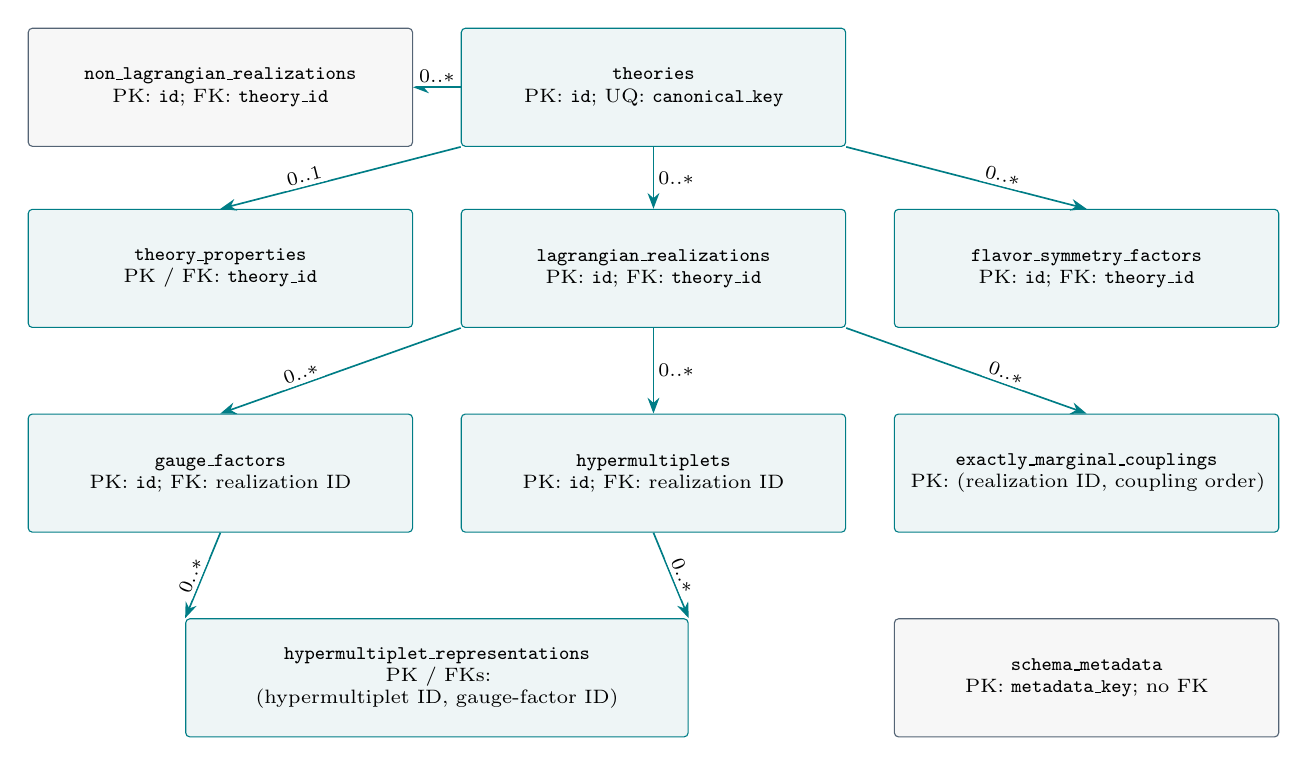
\begin{tikzpicture}[
 entity/.style={draw=accent,fill=pale,rounded corners=1.5pt,
   text width=46mm,minimum height=15mm,inner sep=4pt,align=center,
   font=\scriptsize},
 reserved/.style={entity,draw=muted,fill=black!3},
 relation/.style={-{Stealth[length=2mm]},draw=accent,semithick},
 cardinality/.style={font=\scriptsize\sffamily,fill=white,inner sep=1.5pt}
]
\node[entity] (theories) at (0,0)
 {\texttt{theories}\\PK: \texttt{id}; UQ: \texttt{canonical\_key}};
\node[reserved] (nonlag) at (-5.5,0)
 {\texttt{non\_lagrangian\_realizations}\\PK: \texttt{id}; FK: \texttt{theory\_id}};
\node[entity] (properties) at (-5.5,-2.3)
 {\texttt{theory\_properties}\\PK / FK: \texttt{theory\_id}};
\node[entity] (lagrangian) at (0,-2.3)
 {\texttt{lagrangian\_realizations}\\PK: \texttt{id}; FK: \texttt{theory\_id}};
\node[entity] (flavor) at (5.5,-2.3)
 {\texttt{flavor\_symmetry\_factors}\\PK: \texttt{id}; FK: \texttt{theory\_id}};
\node[entity] (gauge) at (-5.5,-4.9)
 {\texttt{gauge\_factors}\\PK: \texttt{id}; FK: realization ID};
\node[entity] (hypers) at (0,-4.9)
 {\texttt{hypermultiplets}\\PK: \texttt{id}; FK: realization ID};
\node[entity] (couplings) at (5.5,-4.9)
 {\texttt{exactly\_marginal\_couplings}\\PK: (realization ID, coupling order)};
\node[entity,text width=61mm] (representations) at (-2.75,-7.5)
 {\texttt{hypermultiplet\_representations}\\PK / FKs:\\(hypermultiplet ID, gauge-factor ID)};
\node[reserved] (metadata) at (5.5,-7.5)
 {\texttt{schema\_metadata}\\PK: \texttt{metadata\_key}; no FK};
\draw[relation] (theories.west) -- node[cardinality,above] {$0..*$} (nonlag.east);
\draw[relation] (theories.south west) -- node[cardinality,pos=.64,above,sloped] {$0..1$} (properties.north);
\draw[relation] (theories.south) -- node[cardinality,right] {$0..*$} (lagrangian.north);
\draw[relation] (theories.south east) -- node[cardinality,pos=.64,above,sloped] {$0..*$} (flavor.north);
\draw[relation] (lagrangian.south west) -- node[cardinality,pos=.65,above,sloped] {$0..*$} (gauge.north);
\draw[relation] (lagrangian.south) -- node[cardinality,right] {$0..*$} (hypers.north);
\draw[relation] (lagrangian.south east) -- node[cardinality,pos=.65,above,sloped] {$0..*$} (couplings.north);
\draw[relation] (gauge.south) -- node[cardinality,pos=.55,above,sloped] {$0..*$} (representations.north west);
\draw[relation] (hypers.south) -- node[cardinality,pos=.55,above,sloped] {$0..*$} (representations.north east);
\end{tikzpicture}
\end{center}
{\small Arrows run from parent to child; labels give the number of children per
parent allowed by the schema. Each child has exactly one parent along each
foreign key. PK = primary key; FK = foreign key; UQ = unique key. ``Realization
ID'' abbreviates \code{lagrangian_realization_id}. All declared FKs use
\texttt{ON DELETE CASCADE}.}

\subsubsection{How product-group matter is represented}
One \code{hypermultiplets} row holds a complete tensor-product representation
and its submitted \code{kind} and \code{multiplicity}. Its rows in
\code{hypermultiplet_representations} identify the representation under each
gauge factor, including singlets. The latter table joins matter to gauge
factors; it does not create a separate hypermultiplet for each factor.

\begin{note}{Shared flavor versus the submitted matter split}
Schema 6 retains \code{half_hyper_units} in the shared flavor table and JSON,
with $m=2n_{\rm full}+n_{\rm half}$. The original split remains in realization
rows and input/anomaly JSON. Public property-calculator output still reports
both counts; the database strips them from its shared-property copy.
\end{note}

\clearpage
\subsection{Database table catalog and keys}\label{sec:db-tables}
All tables use InnoDB and \code{utf8mb4}. IDs are unsigned \code{BIGINT}s;
standalone \code{id} keys auto-increment. Exact rational values use JSON
numerator/denominator records or separate numeric columns, as detailed below.

{\small
\renewcommand{\arraystretch}{1.17}
\begin{tabularx}{\textwidth}{@{}p{53mm}Y@{}}
\toprule Table & Keys and stored data\\\midrule
\code{schema_metadata} &
PK \code{metadata_key}; \code{metadata_value} holds the schema version
(current value \code{"6"}). Independent of theory rows.\\[3pt]
\code{theories} &
PK \code{id}; UQ \code{canonical_key}. Display name and creation/update
timestamps. A new Lagrangian theory uses \code{lagrangian:<hash>} as its key.\\[3pt]
\code{theory_properties} &
PK/FK \code{theory_id} $\to$ \code{theories.id}. Flavor group/rank/dimension,
conformal-manifold dimension, exact central-charge JSON, separate full-index,
Coulomb-index and Coulomb-spectrum JSON, and combined \code{properties_json}.
Generated, indexed \code{DECIMAL(65,30)} columns approximate $a,c$ for queries.\\[3pt]
\code{flavor_symmetry_factors} &
PK \code{id}; FK \code{theory_id} $\to$ \code{theories.id};
UQ (\code{theory_id}, \code{factor_order}). Group, Lie algebra/rank/dimension,
representation reality, \code{half_hyper_units}, and
\code{gauge_representation_json}. No full/half split columns in schema 6.\\[3pt]
\code{lagrangian_realizations} &
PK \code{id}; FK \code{theory_id} $\to$ \code{theories.id};
UQ \code{canonical_hash} (64-character SHA-256). Gauge group/count, anomaly and
conformality flags, input/anomaly/coupling JSON, creation timestamp.\\[3pt]
\code{non_lagrangian_realizations} &
PK \code{id}; FK \code{theory_id} $\to$ \code{theories.id}. Construction type,
optional source reference, \code{data_json}, creation timestamp. Reserved.\\[3pt]
\code{gauge_factors} &
PK \code{id}; FK realization ID $\to$ \code{lagrangian_realizations.id}.
Separate UQs on (realization ID, \code{factor_order}) and
(realization ID, \code{factor_key}). Group, Cartan type/rank, exact vector,
matter and $b_0$ fractions, beta/global-anomaly flags and Witten parity.\\[3pt]
\code{hypermultiplets} &
PK \code{id}; FK realization ID $\to$ \code{lagrangian_realizations.id};
UQ (realization ID, \code{hyper_order}). Name, \code{kind} (full/half),
submitted multiplicity, total tensor-product dimension and reality.\\[3pt]
\code{hypermultiplet_}\newline\code{representations} &
Composite PK (\code{hypermultiplet_id}, \code{gauge_factor_id}); separate
FKs to \code{hypermultiplets.id} and \code{gauge_factors.id}. Name,
Dynkin-label JSON, dimension/reality, exact Dynkin-index and beta-contribution
numerators/denominators.\\[3pt]
\code{exactly_marginal_couplings} &
Composite PK (realization ID, \code{coupling_order}); FK realization ID
$\to$ \code{lagrangian_realizations.id}. Stores \code{gauge_factor_key}
as text; that key has no additional FK to \code{gauge_factors}.\\\bottomrule
\end{tabularx}}

\subsubsection{Serialization and integrity boundaries}
Full and Coulomb indices are JSON expression strings. Coulomb spectra are
arrays of exact fractions; central charges are exact $a,c$ fraction records.
The separate JSON fields are repeated in \code{properties_json}. Gauge beta
fractions and representation invariants use \code{DECIMAL(65,0)} integer
columns. The writer keeps both ends of each matter--gauge relation within the
same realization; the two individual FKs do not themselves enforce that match.

\clearpage
\subsection{Canonical matter, migrations and import behavior}
The canonical Lagrangian hash is SHA-256 of a normalized payload. Names resolve
to Dynkin labels, repeated matter entries combine, and zero multiplicities
vanish. Conjugate choices use the lexicographically larger label tuple, favoring
fundamentals. Product representations identify only simultaneous conjugation of
all factors. Matter order is ignored; gauge-factor order remains significant.

\subsubsection{Full/half equivalence for pseudoreal representations}
For each complete pseudoreal gauge representation, aggregate before pairing:
\[
 m=2n_{\rm full}+n_{\rm half},\qquad
 (n_{\rm full}^{\rm canonical},n_{\rm half}^{\rm canonical})
 =\bigl(\lfloor m/2\rfloor,\;m\bmod2\bigr).
\]
Four full $SU(2)$ fundamentals, eight halves, or two full plus four halves now
have the same hash. An odd remaining half stays in its own irrep. For products,
the rule uses the reality of the entire tensor product. Real/complex matter
remains full; invalid half-hyper input is rejected by the checker.

\subsubsection{Schema history}
\begin{tabularx}{\textwidth}{@{}p{17mm}Y@{}}
\toprule Migration & Change\\\midrule
$1\to2$ & Add generated, indexed decimal central charges; exact JSON remains
 authoritative.\\
$2\to3$ & Rename the plural full-index property and column to singular
\code{superconformal_index} / \code{superconformal_index_json}.\\
$3\to4$ & Rename the old Coulomb-spectrum/index placeholder to
\code{coulomb_branch_index_json}, including its combined-JSON key.\\
$4\to5$ & Add nullable \code{coulomb_branch_spectrum_json} for actual generator
dimensions; do not compute spectra for existing rows.\\
$5\to6$ & Drop \code{full_hypermultiplets} and \code{half_hypermultiplets}
from \code{flavor_symmetry_factors}; keep \code{half_hyper_units} and the
original realization records.\\\bottomrule
\end{tabularx}

\begin{note}{Schema upgrade and data migration are different operations}
Version 6 does not rehash existing realizations, merge duplicate theories, or
eagerly rewrite old shared JSON. Old hashes from the earlier conjugacy or
full/half conventions require a separate data migration. Under the current
conjugacy convention, inputs already written entirely as full hypers keep their
hashes after full/half normalization.
\end{note}

\code{_insert_shared_properties} ignores the obsolete flavor split when comparing
legacy JSON. Matching JSON is rewritten without that split; a missing Coulomb
spectrum can also be backfilled. Physical property mismatches still raise an
error. Shared flavor metadata retains gauge labels and factor IDs, so this is
not a general comparison of arbitrary dual realizations.

\code{store_lagrangian_theory} checks anomalies/conformality and calculates
properties before looking up the hash. A duplicate returns the existing IDs
with \code{inserted=False}, without updating the realization or calling the
shared-property helper; it therefore does not trigger legacy-JSON cleanup or
spectrum backfill. A new import uses parameterized SQL with commit/rollback.
Schema initialization precedes that DML transaction; MySQL DDL is not covered by
its rollback. No live database was changed for this documentation update.

\clearpage
\section{Package \texttt{test} and reproducible use}\label{sec:test}
\begingroup\small
{\small
\begin{tabularx}{\textwidth}{@{}p{72mm}Y@{}}
\toprule Selected test modules & Main coverage\\\midrule
\code{test_check_n2_anomalies.py} & Root/representation data, all families,
spectator factors, full/half validation, beta and Witten checks.\\
\code{test_n2_theory_index.py} & Laurent output, named/explicit labels, product
singlets, low-order reference indices, LiE parsing and cache concurrency.\\
\code{test_n2_theory_coulomb_branches.py} & Weyl degrees, repeated/fractional
dimensions, PE/PL round trips, relations, full-index projection and precision.\\
\code{test_n2_theory_properties.py} & Flavor blocks, central charges, property
keys, direct gauge-based Coulomb wiring and exact JSON.\\
\code{test_n2_theory_db.py} & Schema/version handling, shared property comparison,
full/half deduplication, legacy JSON/spectrum backfill, SQL parameters and
transactions; actual index equality through $t^6$.\\
\code{test_form_expansion_cache.py} & Exact term serialization, raw-program keys,
thread/process safety, failure behavior and index integration.\\
\code{test_cached_decomposition_planning.py} & Reuse of cached composite blocks,
base identities and consistent serial/parallel dependency planning.\\
\code{test_build_decomposition_cache.py} & Complete enumeration, minimal Adams
calls, parallel batches, resume and CLI contracts.\\\bottomrule
\end{tabularx}}

\subsection{Validation snapshot}
The 10 September 2026 documentation-time rerun of the complete suite finished in
19.658 s: \textbf{209 tests run, 207 passed, 2 skipped}. Backend tests use actual
Sage, FORM and LiE. The two skips require live MySQL; schema migrations and
inserts are otherwise exercised by recording/mocked connections. The index
chapter records exactness comparisons, controlled cache benchmarks and the
limits of the observed speedups. Earlier 134- and 170-test counts describe prior
snapshots and are superseded for the current checkout.

\subsection{Commands and dependencies}
Run from the repository root with Sage's Python, not an unrelated Python
interpreter. FORM and LiE must be discoverable for backend tests.
\begin{lstlisting}[language=bash]
sage -python -m unittest discover -s test -p 'test_*.py' -v
sage -python -m index.n2_theory_index --help
sage -python -m index.char_decomposition_cache --help
sage -python -m common.n2_theory_properties --help
sage -python -m common.n2_theory_db --help
\end{lstlisting}
Sage supplies exact rings and Lie data; FORM and LiE handle expansions and
representation decompositions. PyMySQL supplies the database connection. The
low-level APIs accept executable paths, timeouts and cache paths. The complete
Adams-cache builder lazily imports the OR-Tools-based Frobenius solver; ordinary
index/cache lookups do not require OR-Tools.

\subsection{Practical boundaries before extending the project}
Preserve the exact-number contracts, distinct index/spectrum properties and
source precision. Non-Lagrangian counting needs explicit ring/freeness assumptions;
Higgs work needs an HL/Hilbert-series justification; flavor refinement must
preserve characters through gauge projection. These are mathematical contracts.

\endgroup
\clearpage
\section*{References and equation provenance}
\addcontentsline{toc}{section}{References and equation provenance}
Equation numbers in this document are local. Citations near equations identify
the primary source or software reference; algebraic recurrences, cutoff rules
and function mappings are derived from the inspected project source. Literature
section/equation numbers refer to the linked arXiv editions where specified.
Base software documentation was consulted on 8 September 2026; the new
orthogonality, Sage duality and SQLite references were checked on 10 September. This bibliography
also retains the relevant sources from both earlier summaries.

\begin{thebibliography}{99}
\small\setlength{\itemsep}{8pt}
\bibitem{sage-roots} The Sage Developers, \emph{Root systems}, SageMath reference
manual. Dynkin labels, root/weight lattices and finite Cartan data.
\href{https://doc.sagemath.org/html/en/reference/combinat/sage/combinat/root_system/root_system.html}{Official root-system documentation}.

\bibitem{sage-chars} The Sage Developers, \emph{Weyl character rings}, SageMath
reference manual. Character degrees, duals and Frobenius--Schur indicators.
\href{https://doc.sagemath.org/html/en/reference/combinat/sage/combinat/root_system/weyl_characters.html}{Official Weyl-character documentation}.

\bibitem{bt} L. Bhardwaj and Y. Tachikawa, \emph{Classification of 4d
$\mathcal N=2$ gauge theories}, JHEP 12 (2013) 100, updated arXiv edition.
\href{https://arxiv.org/abs/1309.5160}{arXiv:1309.5160}.
\S2, Eqs.~(2.1)--(2.8): matter, spectator dimensions and beta functions.

\bibitem{lieart} R. Feger, T. W. Kephart and R. J. Saskowski,
\emph{LieART 2.0 -- A Mathematica Application for Lie Algebras and Representation
Theory}, Comput. Phys. Commun. 257 (2020) 107490.
\href{https://arxiv.org/abs/1912.10969}{arXiv:1912.10969}.
Representation tables are cross-checks; LieART is not the project backend.

\bibitem{bilal} A. Bilal, \emph{Lectures on Anomalies}.
\href{https://arxiv.org/abs/0802.0634}{arXiv:0802.0634}.
Chiral anomaly traces, conjugation and product-group anomaly structure.

\bibitem{witten} E. Witten, \emph{An $SU(2)$ Anomaly}, Phys. Lett. B 117
(1982) 324--328.
\href{https://doi.org/10.1016/0370-2693(82)90728-6}{doi:10.1016/0370-2693(82)90728-6}.
Conventional four-dimensional mod-two gauge anomaly.

\bibitem{www} J. Wang, X.-G. Wen and E. Witten, \emph{A New $SU(2)$ Anomaly},
J. Math. Phys. 60 (2019) 052301.
\href{https://arxiv.org/abs/1810.00844}{arXiv:1810.00844}.
\S2.3 includes the conventional isospin parity formula and distinguishes the
additional non-spin anomaly.

\bibitem{df} I. Garc\'ia-Etxebarria and M. Montero,
\emph{Dai--Freed anomalies in particle physics}, JHEP 08 (2019) 003.
\href{https://arxiv.org/abs/1808.00009}{arXiv:1808.00009}.
Global-anomaly scope beyond local anomaly polynomials.

\bibitem{gpr} A. Gadde, E. Pomoni and L. Rastelli,
\emph{The Veneziano Limit of $\mathcal N=2$ Superconformal QCD: Towards the
String Dual of $\mathcal N=2$ $SU(N_c)$ SYM with $N_f=2N_c$},
\href{https://arxiv.org/abs/0912.4918}{arXiv:0912.4918}.
\S5, Eqs.~(5.4)--(5.5), (5.21)--(5.22): the right-index convention and letters.

\bibitem{plethystics} S. Benvenuti, B. Feng, A. Hanany and Y.-H. He,
\emph{Counting BPS Operators in Gauge Theories: Quivers, Syzygies and
Plethystics}, JHEP 11 (2007) 050.
\href{https://arxiv.org/abs/hep-th/0608050}{arXiv:hep-th/0608050}.
\S5: PE, inverse plethystics, complete intersections and refined counting.

\bibitem{lie} M. A. A. van Leeuwen, A. M. Cohen and B. Lisser,
\emph{LiE: A Package for Lie Group Computations} (1992), and LiE reference
manual, character operations (Adams and tensor products).
\href{https://research.tue.nl/en/publications/lie-a-package-for-lie-group-computations}{TU Eindhoven publication record};
\href{https://ir.cwi.nl/pub/29817}{CWI manual record}.

\bibitem{form5} J. A. M. Vermaseren, J. Davies, T. Kaneko, J. Kuipers,
C. Marinissen, B. Ruijl, M. Tentyukov, T. Ueda and J. Vollinga,
\emph{FORM version 5.0.0 Reference manual}, 27 January 2026.
User-supplied \code{form-5.0.0-manual.pdf}; see Chapters 1--3 and the entries
for symbol restrictions, substitution, sorting and rational functions.

\bibitem{form4} J. Kuipers, T. Ueda, J. A. M. Vermaseren and J. Vollinga,
\emph{FORM version 4.0}, Comput. Phys. Commun. 184 (2013) 1453--1467.
\href{https://arxiv.org/abs/1203.6543}{arXiv:1203.6543}.
Software background; FORM 5 syntax is taken from the supplied manual.

\bibitem{sage-degrees} The Sage Developers, \emph{Finite Coxeter groups},
\code{degrees()} documentation. Definition as fundamental invariant degrees,
including product groups and the repeated $D_4$ degree.
\href{https://doc.sagemath.org/html/en/reference/categories/sage/categories/finite_coxeter_groups.html}{Official finite-Coxeter-group documentation}.

\bibitem{st} A. D. Shapere and Y. Tachikawa, \emph{Central charges of
$\mathcal N=2$ superconformal field theories in four dimensions},
JHEP 09 (2008) 109.
\href{https://arxiv.org/abs/0804.1957}{arXiv:0804.1957}.
Eqs.~(2.5)--(2.6): free multiplets; \S3 and Eq.~(5.4): Casimir dimensions and
$4(2a-c)=\sum_i(2\Delta_i-1)$, with stated assumptions.

\bibitem{grry} A. Gadde, L. Rastelli, S. S. Razamat and W. Yan,
\emph{Gauge Theories and Macdonald Polynomials}, Commun. Math. Phys. 319
(2013) 147--193.
\href{https://arxiv.org/abs/1110.3740}{arXiv:1110.3740}.
\S4, Eqs.~(4.5)--(4.11) and (4.15)--(4.17), Appendix B: HL and Coulomb limits.

\bibitem{tachikawa} Y. Tachikawa, \emph{$\mathcal N=2$ supersymmetric dynamics
for pedestrians}, Lecture Notes in Physics 890 (2014).
\href{https://arxiv.org/abs/1312.2684}{arXiv:1312.2684}.
Lagrangian, hypermultiplet, flavor and moduli-space background.

\bibitem{cdi} C. C\'ordova, T. T. Dumitrescu and K. Intriligator,
\emph{Deformations of Superconformal Theories}, JHEP 11 (2016) 135.
\href{https://arxiv.org/abs/1602.01217}{arXiv:1602.01217}.
\S3.2.2/Table 22: four-dimensional $\mathcal N=2$ preserving deformations.

\bibitem{hl-caveat} M. J. Kang, C. Lawrie, K.-H. Lee, M. Sacchi and J. Song,
\emph{Higgs, Coulomb, and Hall--Littlewood}, Phys. Rev. D 106 (2022) 106021.
\href{https://arxiv.org/abs/2207.05764}{arXiv:2207.05764}.
Examples and caveats showing that the HL index and Higgs Hilbert series need
not coincide, including twisted class-S constructions.

\bibitem{stacks} The Stacks Project Authors, \emph{Koszul regular sequences},
\href{https://stacks.math.columbia.edu/tag/062D}{Tag 062D}.
Regular sequences, Koszul homology and exactness criteria used in the
constraint-counting derivation.

\bibitem{hwg} A. Hanany and R. Kalveks, \emph{Highest Weight Generating
Functions for Hilbert Series}, JHEP 10 (2014) 152.
\href{https://arxiv.org/abs/1408.4690}{arXiv:1408.4690}.
Representation-level organization of refined Hilbert series.

\bibitem{etingof} P. Etingof, \emph{Lie Groups and Lie Algebras}, MIT 18.755
lecture notes (2024), Proposition 32.1 (dual highest weights) and Corollary 35.9
(character orthogonality).
\href{https://ocw.mit.edu/courses/18-755-lie-groups-and-lie-algebras-ii-spring-2024/mit18_755_s24_lec_full.pdf}{Official MIT lecture notes}.

\bibitem{sqlite-wal} SQLite, \emph{Write-Ahead Logging}, especially \S2.2
Concurrency. \href{https://www.sqlite.org/wal.html}{Official WAL documentation}.

\bibitem{sqlite-types} SQLite, \emph{Datatypes In SQLite}, \S2 Storage Classes
and Datatypes. \href{https://www.sqlite.org/datatype3.html}{Official datatype documentation}.

\bibitem{python-sqlite} Python Software Foundation, \emph{sqlite3: DB-API 2.0
interface for SQLite databases}; connections, transactions and thread checks.
\href{https://docs.python.org/3/library/sqlite3.html}{Official Python documentation}.
\end{thebibliography}
\end{document}
